% !TEX program = lualatex
\documentclass[11pt,a4paper]{article}

\usepackage{luatexja}
\usepackage{luatexja-fontspec}
\usepackage{amsmath,amssymb}
\usepackage{graphicx}
\usepackage{booktabs}
\usepackage{multirow}
\usepackage{siunitx}
\usepackage{xcolor}
\usepackage[colorlinks=true,linkcolor=blue,citecolor=blue,urlcolor=blue]{hyperref}
\usepackage{longtable}
\usepackage{array}
\usepackage{float}
\usepackage{enumitem}
\usepackage{caption}
\usepackage{subcaption}
\usepackage{geometry}
\usepackage{fancyhdr}
\usepackage{listings}
\usepackage{algorithm}
\usepackage{algpseudocode}
\usepackage{tabularx}
\usepackage{url}
\usepackage{natbib}
\usepackage{appendix}

\captionsetup{font=small,labelfont=bf}
\geometry{margin=25mm}
\setlist{nosep,leftmargin=*}

% Japanese fonts
\setmainjfont{IPAexMincho}
\setsansjfont{IPAexGothic}

\lstset{
  basicstyle=\ttfamily\footnotesize,
  breaklines=true,
  frame=single,
  language=SQL,
  keywordstyle=\color{blue}\bfseries,
  commentstyle=\color{green!50!black},
  stringstyle=\color{red!70!black},
  numbers=left,
  numberstyle=\tiny\color{gray},
  tabsize=2,
}

% =====================================================================
\begin{document}

\title{%
  Schema-Graph-Assisted Text-to-SQL for Materials Databases:\\
  A Method for Natural Language Querying of\\
  Normalized Relational Materials Data\\[6pt]
  \large --- Validated on OQMD Intermetallic Compound Data (B2 and L1$_2$) ---
}
\author{
  Satoshi Minamoto\\
  National Institute for Materials Science (NIMS)\\
  1-2-1 Sengen, Tsukuba, Ibaraki 305-0047, Japan
}
\date{}
\maketitle

% =====================================================================
\begin{abstract}
Materials databases such as the Open Quantum Materials Database (OQMD), Materials Project, and AFLOW
have accumulated vast quantities of first-principles-calculated property data, yet accessing these data
through normalized relational schemas requires SQL expertise that most materials scientists lack.
We present a \textbf{Schema-Graph-Assisted Text-to-SQL (T2SQL) method} that automatically converts
natural language queries into executable SQL statements for normalized materials databases.

The method comprises four key technical components:
(1)~a \textbf{domain-specific entity extractor} with a bilingual (Japanese/English) materials terminology dictionary,
(2)~a \textbf{Schema Graph Traversal Engine} that represents foreign key (FK) relationships as a NetworkX graph
and computes minimal JOIN paths via Steiner tree approximation,
(3)~a \textbf{Few-Shot Retrieval-Augmented Generation (RAG) store} (SQL-as-Few-Shot-Examples)
that accumulates successful NL--SQL pairs and retrieves similar examples via TF-IDF cosine similarity
for LLM prompt injection, including automatic seed example extraction from LaTeX manuscripts, and
(4)~a \textbf{multi-layer SQL Guard} that enforces keyword blacklisting, single-statement restriction,
table whitelisting, and automatic LIMIT injection.

Validation was performed on 909 OQMD intermetallic compounds
(636 B2-type CsCl and 273 L1$_2$-type AuCu$_3$) across 39 test cases
spanning normal queries, absent-data queries, ambiguous/malformed inputs, contradictory conditions,
SQL injection attacks, and safety checks.
A three-level comparison (Naive T2SQL without Schema Graph /
Schema Graph + Rule-based / Schema Graph + GPT-5) demonstrated that
Schema Graph traversal eliminates unnecessary JOINs, correctly handles multi-element AND queries
(which yield zero results under the Naive approach), and achieves Precision = 1.0
against direct OQMD API ground truth for all validated test cases.
The Rule-based mode achieves $<$100~ms latency with zero external API dependency,
while the GPT-5 mode provides superior vocabulary coverage and numeric filter generation
at the cost of $\sim$7.3~s latency and token consumption.

This method lowers the barrier for materials researchers to query normalized relational databases
using natural language.
In the emerging paradigm of AI for Science (AI4S), where AI is expected to accelerate
every stage of the scientific workflow---from hypothesis generation through data retrieval
to experimental design---the ability to access structured materials data
via natural language constitutes critical infrastructure.
This work contributes to the democratization of data utilization in materials informatics
and provides a foundational building block for AI4S-driven materials discovery.

\vspace{6pt}
\noindent\textbf{Keywords:}
Text-to-SQL, materials database, schema graph, Retrieval-Augmented Generation,
OQMD, intermetallic compounds, natural language processing, materials informatics, AI for Science
\end{abstract}

% =====================================================================
\tableofcontents
\newpage

% =====================================================================
\section{Introduction}
\label{sec:introduction}

\subsection{AI for Science and the Data Access Barrier in Materials Informatics}

The paradigm of \textbf{AI for Science (AI4S)}---the systematic application of
artificial intelligence to accelerate scientific discovery---is transforming
materials research~\citep{wang2023ai4s}.
AI4S envisions an integrated workflow where AI agents autonomously
generate hypotheses, retrieve relevant data from large-scale databases,
design experiments or simulations, and interpret results.
Within this vision, \textbf{natural language access to structured materials data}
is not merely a convenience but a prerequisite:
if AI agents (or the researchers directing them) cannot efficiently query
normalized relational databases, the entire AI4S pipeline is bottlenecked
at the data retrieval stage.

The rapid growth of high-throughput first-principles calculations has produced
several large-scale materials databases:
the Open Quantum Materials Database (OQMD, $\sim$1M entries)~\citep{saal2013oqmd,kirklin2015oqmd},
the Materials Project ($>$150K entries)~\citep{jain2013mp},
AFLOW ($>$3.5M entries)~\citep{curtarolo2012aflow}, and
NOMAD~\citep{draxl2019nomad}.
These databases are indispensable for computational materials discovery,
screening of candidate phases~\citep{senkov2018hea,george2019hea},
and validation of experimental observations.

However, accessing data stored in normalized relational schemas (multiple tables
connected by foreign keys) requires SQL expertise.
For example, querying ``stable B2 compounds containing Fe with their lattice constants''
on a properly normalized schema demands a 4-table JOIN with WHERE conditions
on element, prototype, and thermodynamic stability---a query that is straightforward for
database engineers but non-trivial for materials scientists.

While REST APIs (such as OQMD's \texttt{/oqmdapi/formationenergy}) partially address this barrier,
they impose their own learning curve (filter syntax, pagination handling, response parsing)
and lack the flexibility of arbitrary SQL queries over locally curated datasets.

In the AI4S context, this data access barrier is particularly critical:
autonomous AI agents performing materials screening or property prediction
must issue complex, multi-condition database queries programmatically.
A natural language interface that reliably generates correct SQL
enables both human researchers and AI agents to interact with materials databases
without database engineering expertise,
thereby removing a key bottleneck in the AI4S workflow.

\subsection{Text-to-SQL: State of the Art}

Text-to-SQL (T2SQL) research has advanced rapidly with large-scale benchmarks:
Spider~\citep{yu2018spider} (10,181 questions, 200 databases, 138 domains) and
BIRD~\citep{li2024bird} (12,751 questions, 95 databases, 33.4~GB).
Recent LLM-based methods achieve high accuracy:
DAIL-SQL~\citep{gao2023dail} reports 86.6\% execution accuracy on Spider using
skeleton-based few-shot example selection,
and DIN-SQL~\citep{pourreza2024dinsql} achieves 85.3\% using decomposed in-context learning.
\citet{hong2024survey} provide a comprehensive survey noting the dominant role of schema linking.
\citet{maamari2024schema} argue that advanced LLMs may render explicit schema linking unnecessary,
though this remains debated.

However, \textbf{all existing T2SQL benchmarks target general-purpose domains}
(e-commerce, healthcare, education), and no prior work has addressed
the specific challenges of materials science databases:
domain-specific terminology (Strukturbericht designations, prototype names),
bilingual queries (Japanese/English element names),
composition table normalization (one row per element per compound), and
thermodynamic stability filters ($E_\text{hull} \leq 0.001$~eV/atom).

\subsection{NLP in Materials Informatics}

NLP applications in materials science are expanding:
MatSci-NLP~\citep{song2023matscnlp} benchmarks 7 NLP tasks on materials text,
LLAMAT~\citep{mishra2024llamat} improves information extraction via continual pre-training of LLaMA,
the Materials Knowledge Navigation Agent (MKNA)~\citep{zhuang2026mkna} translates
natural language intent into database retrieval and structure generation actions,
and OptiMat Alloys~\citep{hu2026optimat} provides an LLM-powered conversational alloy explorer.
Materials Project has begun offering MCP-based LLM integration.

These works address information extraction and agent-based database interaction,
but \textbf{none target schema-aware SQL generation on normalized relational databases}---specifically,
automatic JOIN path discovery through foreign key graph traversal.
This gap is the focus of our method.

\subsection{Objectives and Novelty}

Our contributions are threefold:

\begin{enumerate}
  \item \textbf{A materials-domain-specific Schema Graph T2SQL method}
    combining a bilingual materials terminology dictionary with FK relationship graph traversal
    for automatic JOIN path computation on normalized materials databases.
  \item \textbf{SQL-as-Few-Shot-Examples with manuscript-based seed extraction}:
    a RAG feedback loop that accumulates successful NL--SQL pairs
    and retrieves them via TF-IDF similarity for LLM prompt injection,
    with automatic seed example extraction from LaTeX research papers.
  \item \textbf{Integration test methodology using OQMD API ground truth}:
    quantitative validation of the entire data pipeline
    (API $\to$ CSV $\to$ RDB normalization $\to$ NL $\to$ SQL $\to$ JOIN reconstruction)
    using Precision/Recall against direct API queries.
\end{enumerate}

% =====================================================================
\section{Methods}
\label{sec:methods}

This section describes each technical component in detail.
The overall pipeline architecture is shown in Fig.~\ref{fig:architecture}.

\begin{figure}[htbp]
  \centering
  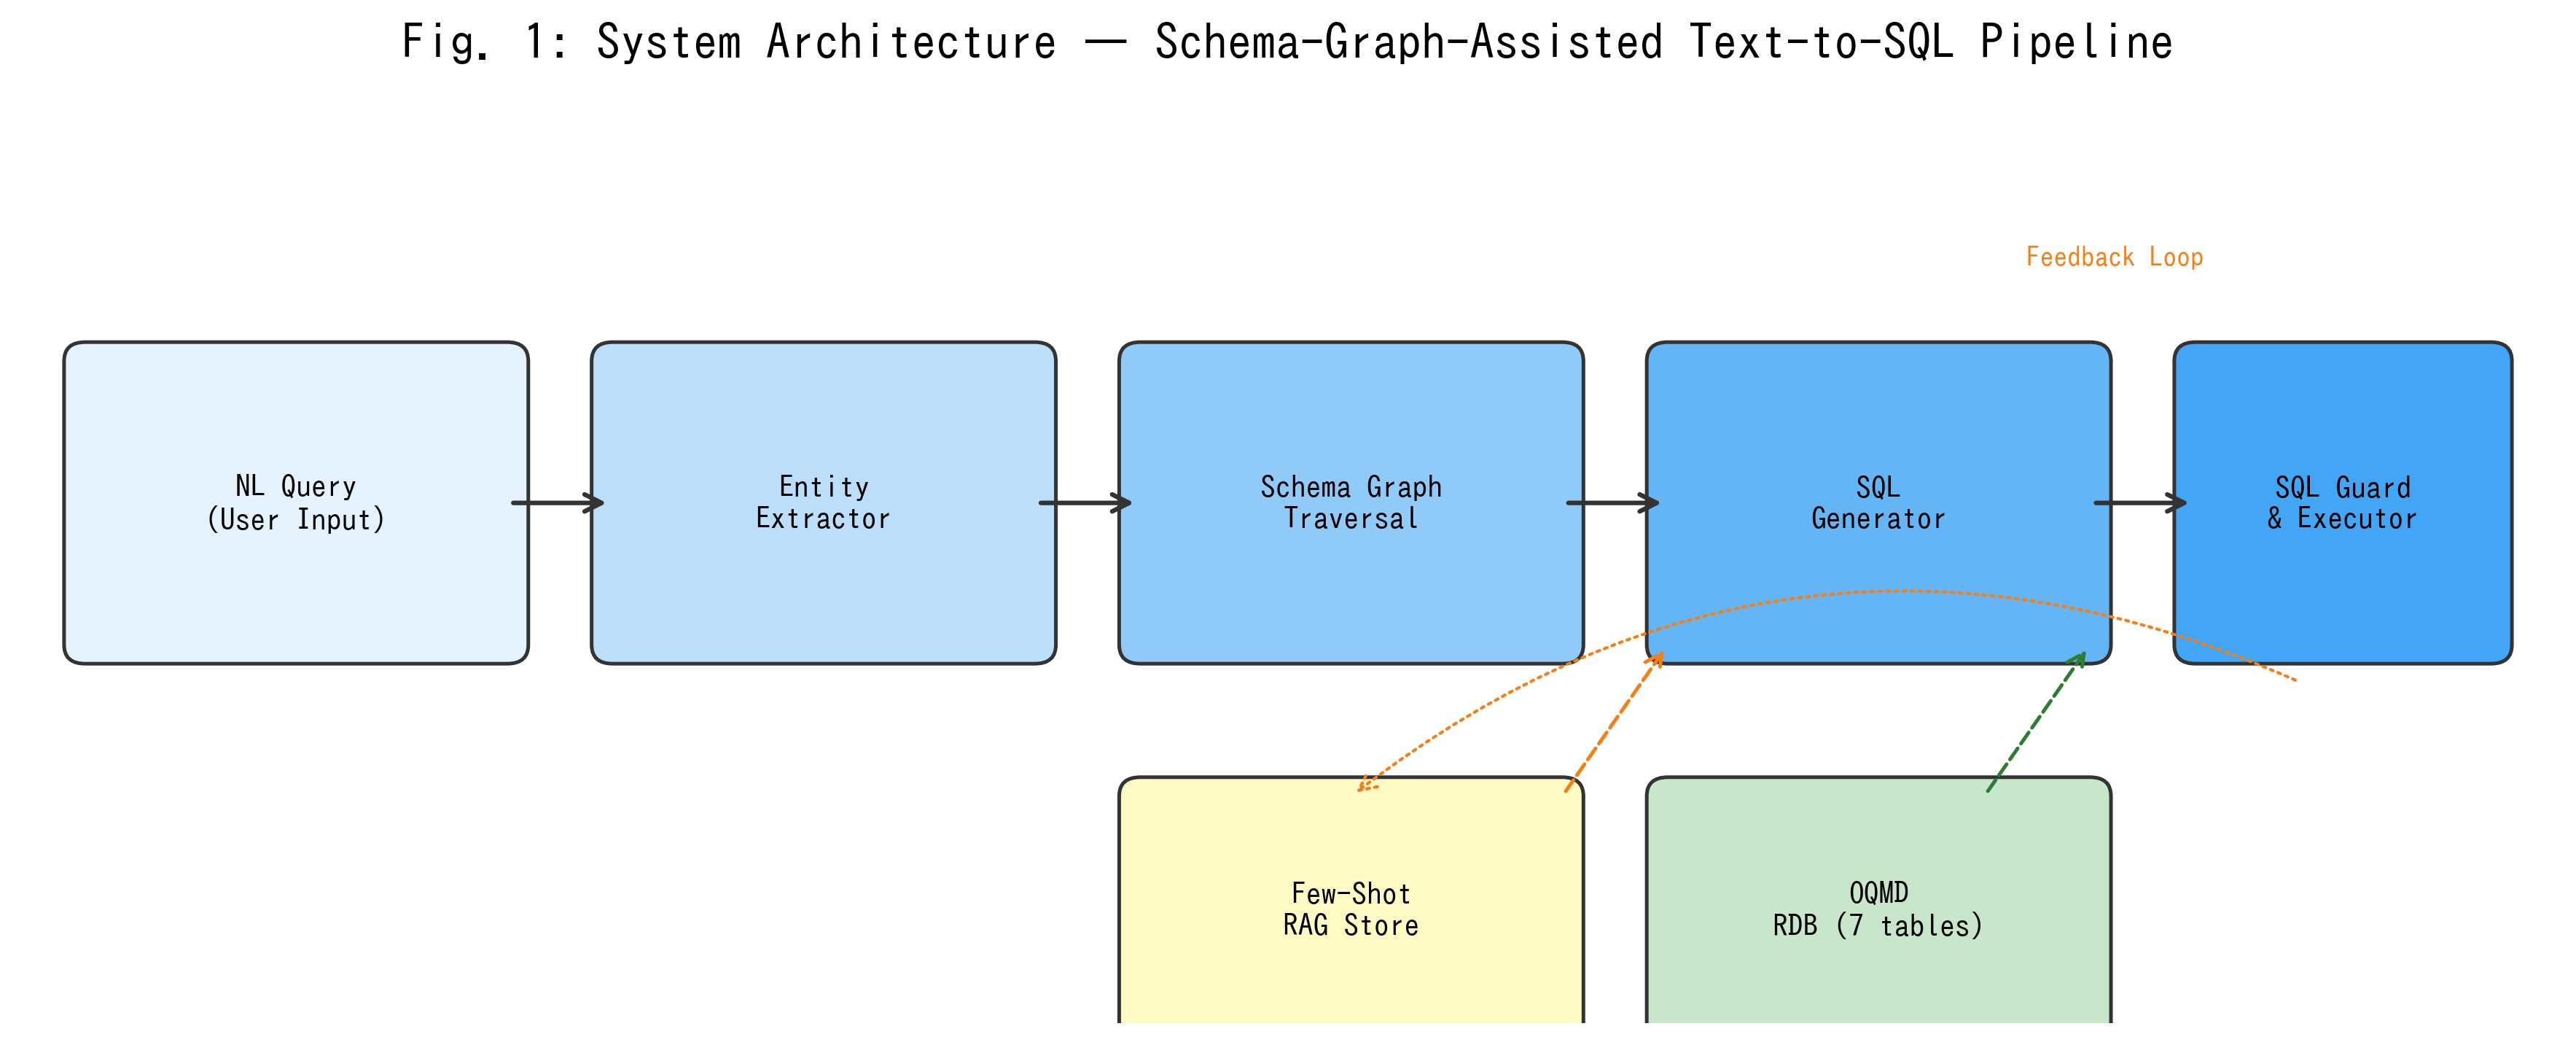
\includegraphics[width=\linewidth]{figures/fig1_architecture.png}
  \caption{System architecture of the Schema-Graph-Assisted Text-to-SQL pipeline.
    Solid arrows indicate the primary data flow; dashed arrows indicate the
    Few-Shot RAG feedback loop (successful query pairs are stored and retrieved for future queries).
    The SQL Guard acts as a final safety layer before database execution.}
  \label{fig:architecture}
\end{figure}

\subsection{Database Schema Design for Materials Data}
\label{sec:schema_design}

\subsubsection{Normalization of OQMD Data into a 7-Table Schema}

OQMD's REST API returns flat JSON records (one entry = one JSON object),
which we normalize into a 7-table relational schema (Fig.~\ref{fig:er_diagram}, Table~\ref{tab:schema}).
The design follows Boyce-Codd Normal Form (BCNF) and is motivated by the following materials-domain considerations:

\begin{figure}[htbp]
  \centering
  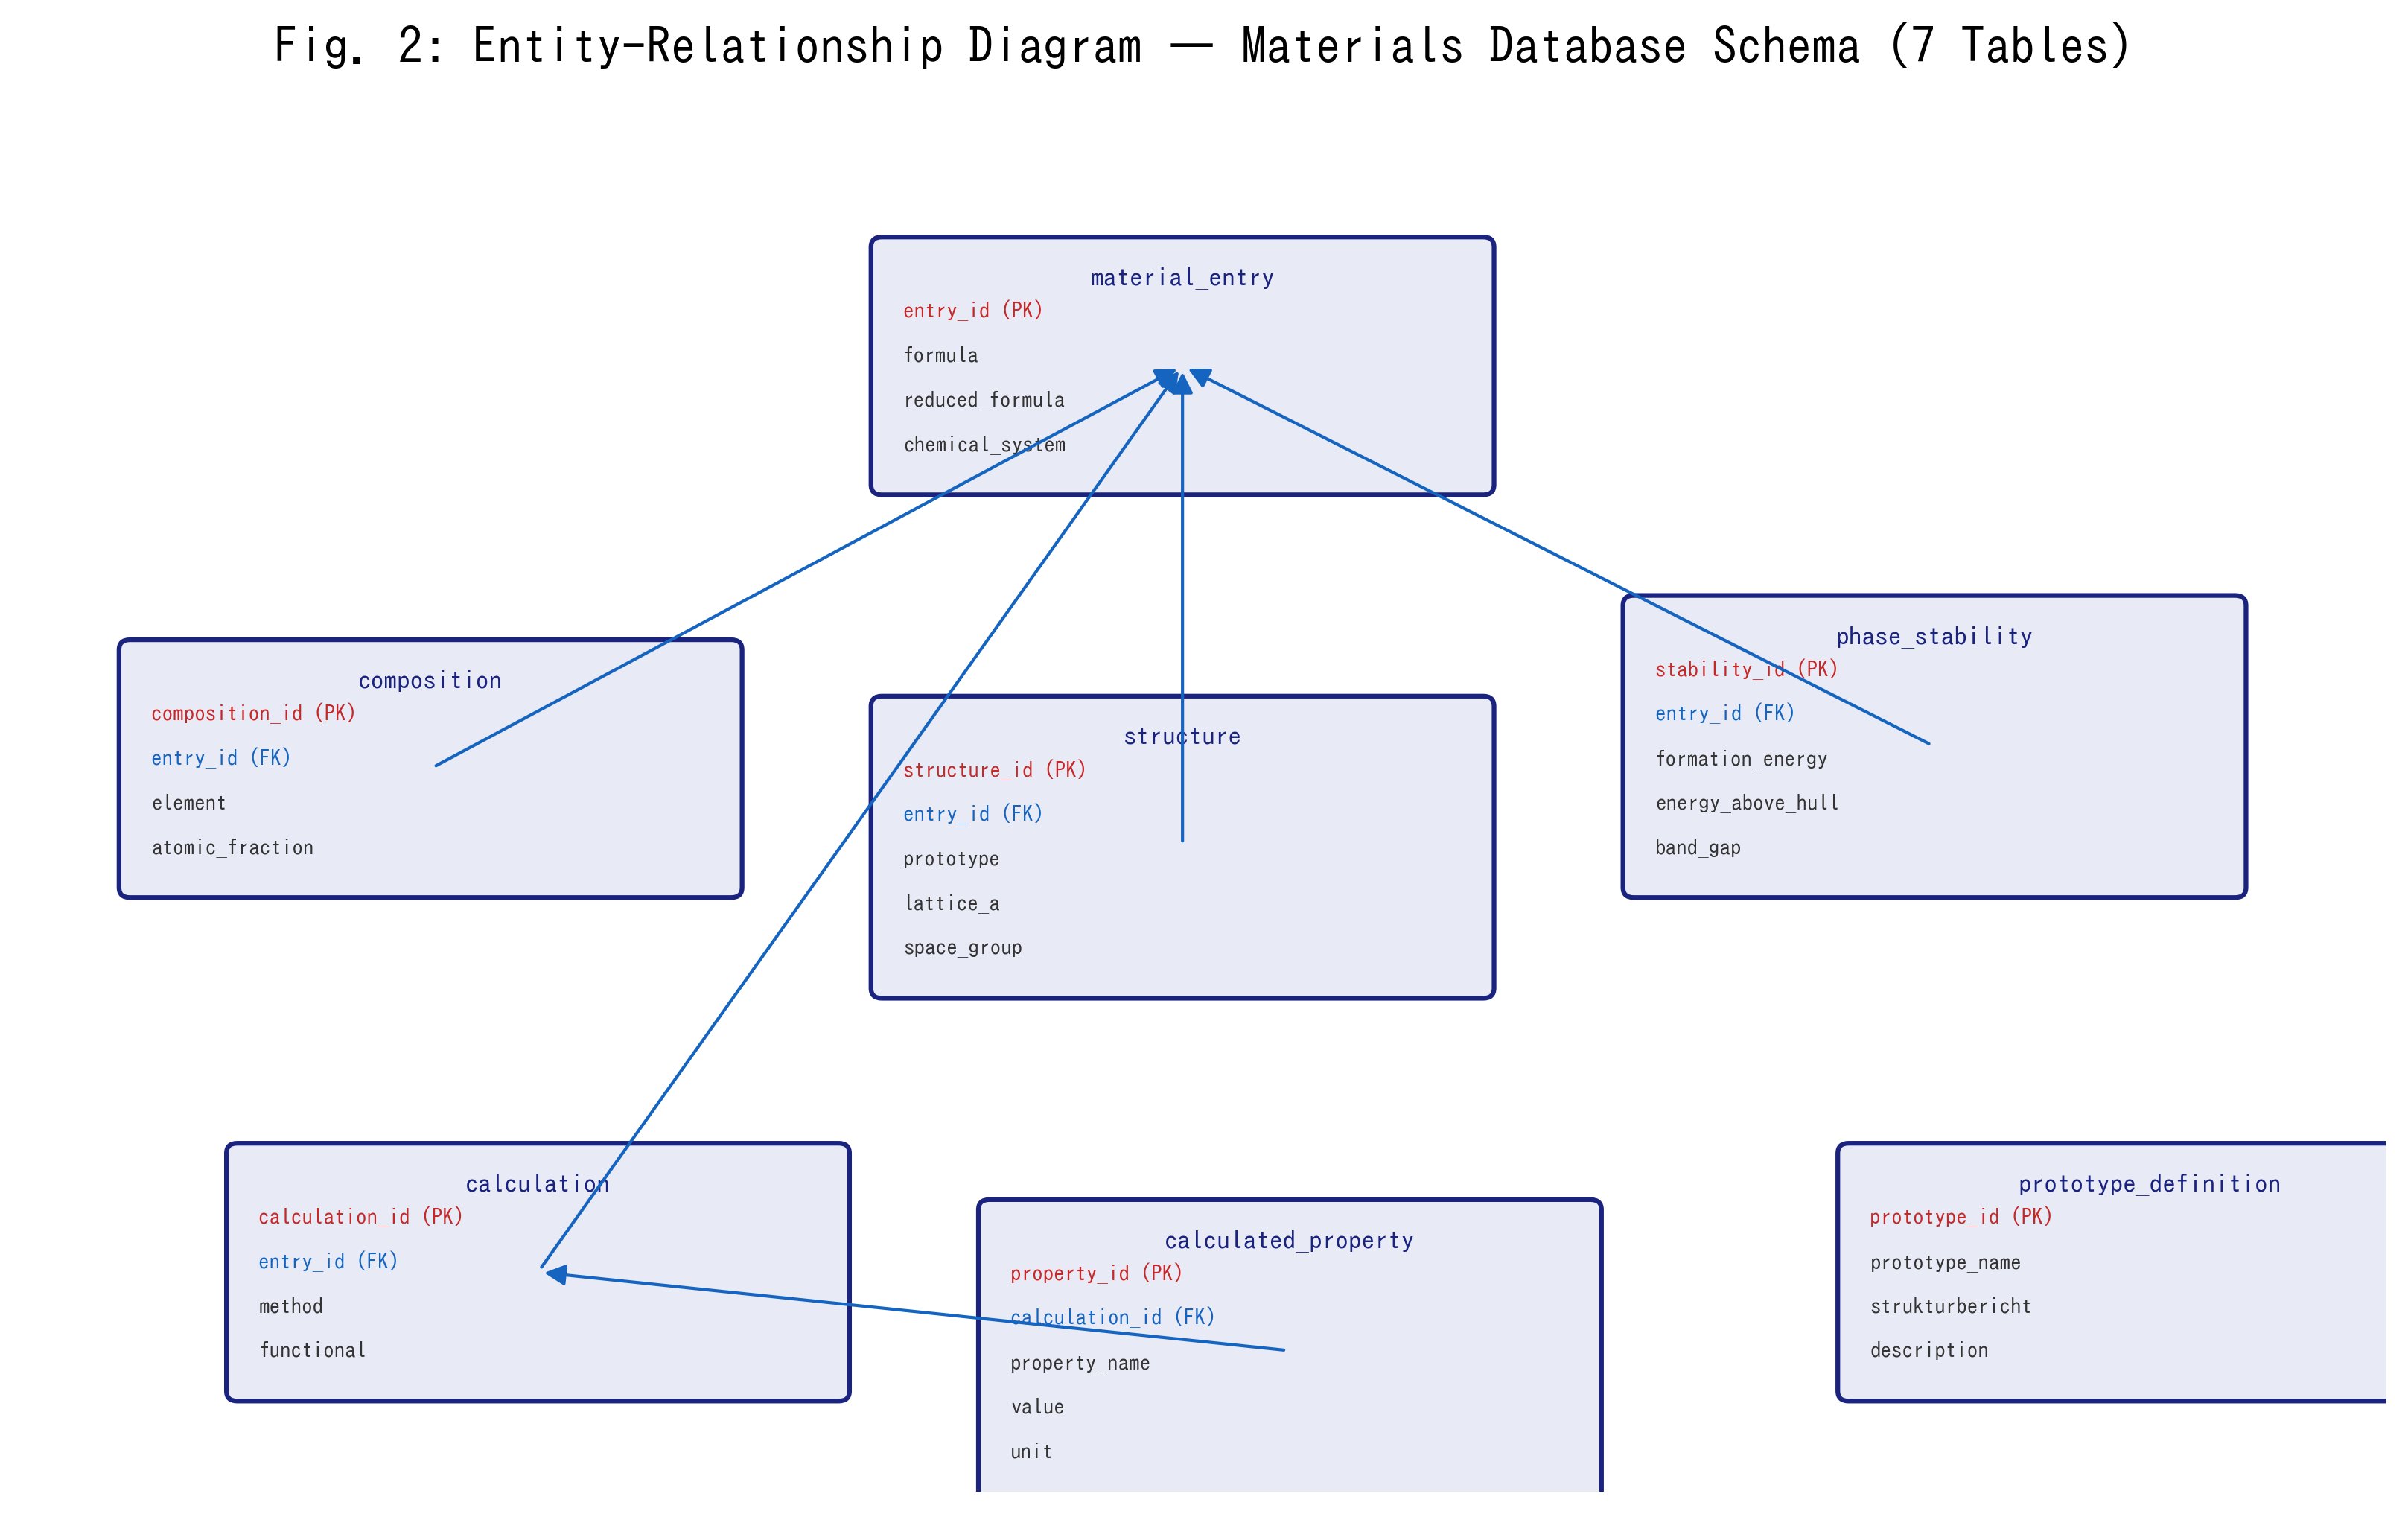
\includegraphics[width=0.9\linewidth]{figures/fig2_er_diagram.png}
  \caption{Entity-Relationship diagram of the 7-table materials database schema.
    All tables are connected to \texttt{material\_entry} via foreign keys (blue lines).
    Red = primary key, Blue = foreign key.}
  \label{fig:er_diagram}
\end{figure}

\begin{table}[htbp]
  \centering
  \caption{Database schema overview (7 tables).}
  \label{tab:schema}
  \small
  \begin{tabularx}{\linewidth}{lllX}
    \toprule
    Table & PK & FK & Key Columns \\
    \midrule
    material\_entry & entry\_id & --- & formula, reduced\_formula, chemical\_system \\
    composition & composition\_id & entry\_id & element, atomic\_fraction \\
    structure & structure\_id & entry\_id & prototype, strukturbericht, lattice\_a, space\_group \\
    phase\_stability & stability\_id & entry\_id & formation\_energy\_per\_atom, energy\_above\_hull, band\_gap \\
    calculation & calculation\_id & entry\_id & method, functional \\
    calculated\_property & property\_id & calculation\_id & property\_name, value, unit \\
    prototype\_definition & prototype\_id & --- & prototype\_name, strukturbericht, description \\
    \bottomrule
  \end{tabularx}
\end{table}

\paragraph{Composition table separation.}
A single compound may contain multiple elements (e.g., Fe$_3$Al $\to$ Fe and Al).
By storing each element as a separate row in the \texttt{composition} table,
we enable flexible element-based queries (AND, OR, NOT) without string parsing.
This normalization, however, introduces a critical complexity:
a query for ``compounds containing both Ni and Al'' cannot use a simple
\texttt{WHERE element = 'Ni' AND element = 'Al'} (which would return zero rows,
since no single row contains both elements simultaneously).
Instead, \texttt{EXISTS} subqueries are required (see Section~\ref{sec:multi_element}).

\paragraph{Structure/Phase stability/Calculation separation.}
Crystal structure information (prototype, lattice constant), thermodynamic stability
(energy above hull), and calculation metadata (DFT functional) are stored in separate tables
to allow independent updates and extensions.

\paragraph{Entity-Attribute-Value (EAV) for calculated properties.}
The \texttt{calculated\_property} table uses an EAV pattern (\texttt{property\_name}, \texttt{value}, \texttt{unit})
to accommodate arbitrary computed properties (bulk modulus, shear modulus, etc.)
without schema modifications.

\subsubsection{XML/YAML Representation for RAG Context Injection}

The schema structure is serialized as YAML (\texttt{allowed\_schema.yaml}),
which serves dual purposes:
(a) the SQL Guard's table/column whitelist (Section~\ref{sec:sql_guard}), and
(b) RAG context for LLM prompts---the schema YAML is injected into the system message
so the LLM understands available tables, columns, and their types.
This approach is analogous to schema serialization techniques used in
general T2SQL~\citep{gao2023dail}, but here specialized for materials databases
with domain-specific column semantics (e.g., \texttt{energy\_above\_hull} represents $E_\text{hull}$).

\subsection{Entity Extractor with Materials Terminology Dictionary}
\label{sec:entity_extractor}

The entity extractor converts natural language queries into structured condition dictionaries
using a YAML-based bilingual terminology dictionary (\texttt{material\_terms.yaml}).

\subsubsection{Dictionary Structure}

The dictionary contains four categories:

\begin{enumerate}
  \item \textbf{Prototype aliases}: Mapping between prototype names and their variants.\\
    Example: \texttt{B2} $\leftrightarrow$ [\texttt{B2}, \texttt{CsCl}, \texttt{CsCl型}, \texttt{B2型}]\\
    \texttt{L12} $\leftrightarrow$ [\texttt{L1$_2$}, \texttt{L12}, \texttt{AuCu3}, \texttt{Cu$_3$Au型}, \texttt{$\gamma'$}]

  \item \textbf{Element mappings}: Symbol $\leftrightarrow$ Japanese/English name correspondence.\\
    Example: \texttt{Fe} $\leftrightarrow$ [\texttt{Fe}, \texttt{鉄 (tetsu)}, \texttt{iron}]

  \item \textbf{Stability terms}: Natural language $\to$ numerical threshold.\\
    ``stable'' / ``安定'' $\to$ \texttt{energy\_above\_hull} $\leq 0.001$~eV/atom\\
    ``metastable'' / ``準安定'' $\to$ \texttt{energy\_above\_hull} $\leq 0.05$~eV/atom

  \item \textbf{Property terms}: Mapping property descriptions to table.column references.\\
    ``lattice constant'' / ``格子定数'' $\to$ \texttt{structure.lattice\_a}\\
    ``formation energy'' / ``形成エネルギー'' $\to$ \texttt{phase\_stability.formation\_energy\_per\_atom}
\end{enumerate}

\subsubsection{Unicode Normalization and Pattern Matching}

Unicode subscript characters (₀₁₂₃₄₅₆₇₈₉) are normalized to ASCII digits before matching.
Element symbol recognition uses word-boundary regular expressions to correctly distinguish
standalone ``Fe'' from ``FeCoNi'' substrings.

\subsubsection{Output Format}

The extractor returns a structured dictionary:

\begin{lstlisting}[language=Python,caption={Entity extraction example.},label=lst:extract]
# Input: "Show stable B2 compounds containing Fe"
# Output:
{
  "prototype": "B2",
  "contains_elements": ["Fe"],
  "stability": "stable",
  "sort_by": None,
  "sort_order": None
}
\end{lstlisting}

\subsection{Schema Graph Traversal Engine}
\label{sec:schema_graph}

This is the core algorithmic contribution of the proposed method.
The engine represents the database schema as a graph and computes optimal JOIN paths automatically.

\subsubsection{Graph Construction from PostgreSQL Metadata}

Foreign key relationships are extracted dynamically from PostgreSQL's \texttt{information\_schema}:

\begin{lstlisting}[language=SQL,caption={FK relationship extraction query.},label=lst:fk_query]
SELECT tc.table_name AS source_table,
       kcu.column_name AS source_column,
       ccu.table_name AS target_table,
       ccu.column_name AS target_column
  FROM information_schema.table_constraints tc
  JOIN information_schema.key_column_usage kcu
    ON tc.constraint_name = kcu.constraint_name
  JOIN information_schema.constraint_column_usage ccu
    ON ccu.constraint_name = tc.constraint_name
 WHERE tc.constraint_type = 'FOREIGN KEY'
   AND tc.table_schema = 'public';
\end{lstlisting}

The result is stored as an undirected NetworkX~\citep{networkx2008} graph $G = (V, E)$
where $V$ = \{table names\} and $E$ = \{FK relationships\}.
Because FK metadata is read at runtime, the graph automatically adapts to schema changes
without code modifications.

\subsubsection{Minimal Covering JOIN Path: Steiner Tree Approximation}
\label{sec:steiner}

Given a set of \textit{required tables} $R \subseteq V$ (determined by the entity extractor's output),
we need the minimum subgraph of $G$ that connects all tables in $R$.
This is the Steiner tree problem in graphs~\citep{hwang1992steiner}, which is NP-hard in general.

For our 7-node, 6-edge schema graph, we employ a greedy heuristic
(Algorithm~\ref{alg:steiner}) that is exact for tree-structured graphs
(which our FK graph is):

\begin{algorithm}[htbp]
  \caption{Minimal covering JOIN subgraph (Steiner tree approximation).}
  \label{alg:steiner}
  \begin{algorithmic}[1]
    \Require FK relationship graph $G = (V, E)$, required table set $R$
    \Ensure List of JOIN paths $P$
    \State $P \gets \emptyset$, $\text{covered} \gets \emptyset$
    \ForAll{$(s, t) \in \binom{R}{2}$}
      \If{$s \in \text{covered} \land t \in \text{covered}$}
        \State \textbf{continue} \Comment{Both endpoints already connected}
      \EndIf
      \State $p \gets \text{ShortestPath}(G, s, t)$ \Comment{BFS on FK graph}
      \If{$p \neq \emptyset$}
        \State $P \gets P \cup \{p\}$
        \State $\text{covered} \gets \text{covered} \cup \text{nodes}(p)$
      \EndIf
    \EndFor
    \ForAll{$r \in R \setminus \text{covered}$} \Comment{Handle isolated required tables}
      \State $c \gets $ nearest node in covered
      \State $P \gets P \cup \{\text{ShortestPath}(G, r, c)\}$
    \EndFor
    \State \Return $P$
  \end{algorithmic}
\end{algorithm}

\paragraph{Complexity.}
For a graph with $|V| = n$ nodes and $|R| = k$ required tables,
the algorithm performs $O(k^2)$ shortest-path computations, each $O(n + |E|)$ via BFS.
For our schema ($n = 7$, $k \leq 5$), this completes in microseconds.

\paragraph{Correctness for tree-structured FK graphs.}
When $G$ is a tree (as in our schema, where \texttt{material\_entry} is the hub),
the Steiner tree is unique and our greedy algorithm finds it exactly.
For schemas with FK cycles (e.g., self-referencing tables), the approximation
may include unnecessary edges, but this is acceptable for SQL generation
(extra JOINs increase query cost but do not affect correctness if DISTINCT is applied).

\subsubsection{JOIN Path $\to$ SQL FROM/JOIN Clause Generation}

Each path in $P$ is converted to SQL JOIN clauses.
The FK metadata provides the join column names:

\begin{lstlisting}[language=Python,caption={JOIN clause generation from path.},label=lst:join_gen,numbers=none]
# Path: [material_entry, structure]
# FK: structure.entry_id -> material_entry.entry_id
# Generated:
#   FROM material_entry m
#   JOIN structure s ON s.entry_id = m.entry_id
\end{lstlisting}

Table aliases are assigned automatically (first letter of table name,
with conflict resolution for collisions).

\subsubsection{Multi-Element AND Query: The EXISTS Subquery Pattern}
\label{sec:multi_element}

A critical materials-specific challenge arises from the composition table normalization.
Querying ``compounds containing both Ni and Al'' requires:

\begin{lstlisting}[language=SQL,caption={Multi-element AND query using EXISTS subqueries.},label=lst:exists]
SELECT DISTINCT m.entry_id, m.formula
FROM material_entry m
WHERE EXISTS (
    SELECT 1 FROM composition
    WHERE entry_id = m.entry_id AND element = 'Ni')
  AND EXISTS (
    SELECT 1 FROM composition
    WHERE entry_id = m.entry_id AND element = 'Al')
LIMIT 100;
\end{lstlisting}

The Schema Graph engine detects when multiple elements are specified
and automatically generates EXISTS subqueries instead of direct JOINs.
Without this pattern (Naive approach), the query
\texttt{WHERE c.element = 'Ni' AND c.element = 'Al'}
returns zero rows because no single composition row can satisfy both conditions simultaneously.
This is the \textbf{most critical failure mode} prevented by the Schema Graph method.

\subsubsection{Comparison: Naive vs. Schema Graph (Worked Example)}

Table~\ref{tab:naive_vs_sg} illustrates the difference for query
``Show B2 compounds containing Fe'':

\begin{table}[htbp]
  \centering
  \caption{SQL generation comparison: Naive vs. Schema Graph for ``B2 compounds containing Fe''.}
  \label{tab:naive_vs_sg}
  \small
  \begin{tabularx}{\linewidth}{lXX}
    \toprule
    Aspect & Naive (Level 0) & Schema Graph (Level 1) \\
    \midrule
    JOIN tables & All 6 tables always & Only composition + structure (2 tables) \\
    JOIN count & 5 JOINs & 2 JOINs \\
    DISTINCT & No $\to$ duplicate rows & Yes \\
    LIMIT & No $\to$ unbounded & Yes (100) \\
    Safety validation & No & Full (keyword + table whitelist) \\
    Multi-element AND & Incorrect (0 rows) & Correct (EXISTS) \\
    \bottomrule
  \end{tabularx}
\end{table}

\subsection{SQL Generation: Rule-based and LLM Modes}
\label{sec:sql_generation}

The system supports two SQL generation modes, both operating within the
Schema Graph constraints:

\subsubsection{Rule-based Mode (Level 1)}

A deterministic template-based generator constructs SQL from the extracted conditions
and Schema Graph JOIN paths.
No external API is required; latency is $<$100~ms.
Limitations: cannot generate numeric comparison WHERE clauses
(e.g., \texttt{band\_gap > 1.0}), cannot handle negation
(``compounds \textit{not} containing Fe''), and cannot understand
terminology not in the dictionary.

\subsubsection{LLM Mode with Few-Shot RAG (Level 2)}
\label{sec:llm_mode}

When the Rule-based mode's dictionary coverage is insufficient
(e.g., unregistered elements, numeric conditions, complex phrasing),
the system falls back to LLM-based generation.
The LLM (GPT-5 in our experiments) receives a structured prompt containing:

\begin{enumerate}
  \item \textbf{System message}: Task description + Schema YAML (table names, column names, types, FK relationships)
  \item \textbf{Few-Shot examples}: Top-$k$ similar NL--SQL pairs from the RAG store (Section~\ref{sec:few_shot})
  \item \textbf{User message}: The natural language query
  \item \textbf{Constraints}: ``Generate only SELECT statements'', ``Include LIMIT 100'',
        ``Use only tables listed in the schema''
\end{enumerate}

The generated SQL is then validated by the SQL Guard (Section~\ref{sec:sql_guard})
before execution.

\subsection{Few-Shot RAG Store (SQL-as-Few-Shot-Examples)}
\label{sec:few_shot}

\subsubsection{Architecture}

The Few-Shot store implements a RAG~\citep{lewis2020rag} pattern specialized for T2SQL:

\begin{enumerate}
  \item \textbf{Accumulation}: When a query successfully produces results,
    the (NL query, SQL, conditions, row count, source) tuple is appended to a JSON store.
  \item \textbf{Retrieval}: For a new query, TF-IDF~\citep{salton1988tfidf} cosine similarity
    is computed against all stored NL queries, and the top-$k$ (default $k=3$) are returned.
  \item \textbf{Injection}: Retrieved examples are formatted as
    ``\texttt{Question: ... SQL: ...}'' blocks and prepended to the LLM prompt.
\end{enumerate}

\subsubsection{TF-IDF Tokenization for Materials Queries}

Standard NLP tokenizers are inadequate for materials queries because they split
chemical formulas and element symbols incorrectly.
Our tokenizer uses a combined regex pattern:

\begin{lstlisting}[language=Python,caption={TF-IDF tokenizer for materials queries.},label=lst:tokenizer,numbers=none]
# Tokenization pattern:
# 1. Chemical symbols: [A-Z][a-z]? (Fe, Ni, Al, ...)
# 2. Japanese characters: [\u3040-\u9fff]+
# 3. English words: [a-z]+
# 4. Numbers: \d+
tokens = re.findall(
  r'[A-Z][a-z]?|[\u3040-\u9fff]+|[a-z]+|\d+',
  query.lower()
)
\end{lstlisting}

IDF is computed using $\text{IDF}(t) = \log(N / n_t)$ where $N$ is the total number of
stored examples and $n_t$ is the number containing term $t$.
Cosine similarity between query and stored example TF-IDF vectors determines ranking.

\subsubsection{Seed Example Extraction from Research Papers}

To bootstrap the Few-Shot store without manual curation,
we implemented automatic seed example extraction from LaTeX manuscripts.
The extractor scans for patterns such as:

\begin{itemize}
  \item \texttt{B2[-\\s]type\\s*(formula)} $\to$ \{prototype: B2, elements: extracted\}
  \item \texttt{L1[\$\_\{\}2]+[-\\s]*(formula)} $\to$ \{prototype: L12, elements: extracted\}
  \item Context keywords within 100 characters: ``lattice'', ``stable'', ``formation energy''
\end{itemize}

For each extracted compound mention, a canonical NL query and corresponding SQL are generated.
In our experiments, 4 seed examples were automatically extracted from
\texttt{hea\_lattice\_prediction.tex}, complementing 7 manually curated examples
(11 total; Table~\ref{tab:few_shot_sources}).

\begin{table}[htbp]
  \centering
  \caption{Few-Shot store composition (11 examples).}
  \label{tab:few_shot_sources}
  \small
  \begin{tabular}{lccl}
    \toprule
    Source & Count & \% & Example Query \\
    \midrule
    Manual curation & 7 & 64\% & ``Show B2 compounds containing Fe'' \\
    Paper extraction & 4 & 36\% & ``Show properties of B2 FeAl'' \\
    \bottomrule
  \end{tabular}
\end{table}

\subsection{SQL Guard: Multi-layer Safety Validation}
\label{sec:sql_guard}

All generated SQL---whether from Rule-based or LLM mode---passes through
a 5-layer validation pipeline before database execution:

\begin{enumerate}
  \item \textbf{Multiple statement detection}: Reject if semicolons appear within the SQL body
    (prevents piggyback attacks such as \texttt{SELECT ...; DROP TABLE ...}).
  \item \textbf{Forbidden keyword detection}: Scan for INSERT, UPDATE, DELETE, DROP, ALTER,
    TRUNCATE, CREATE, GRANT, REVOKE, COPY using word-boundary regex matching.
  \item \textbf{SELECT-only restriction}: Reject any statement not beginning with SELECT or WITH.
  \item \textbf{Table whitelist verification}: Extract all table names referenced in FROM/JOIN clauses
    and verify each appears in \texttt{allowed\_schema.yaml}.
    Queries referencing undeclared tables (e.g., \texttt{secret\_passwords}) are rejected.
  \item \textbf{Automatic LIMIT injection}: If no LIMIT clause is present, append \texttt{LIMIT 100}
    to prevent unbounded result sets from consuming excessive memory or computation.
\end{enumerate}

Optionally, SQLGlot~\citep{sqlglot2023} performs AST-level syntax validation
(detecting structurally malformed SQL that passes regex checks).

\subsection{Recommended Operational Configuration: Cascading Mode}
\label{sec:cascade}

Based on the characteristics of each generation mode, we recommend a cascading strategy:

\begin{enumerate}
  \item \textbf{Stage 1}: Attempt Rule-based generation (Level 1, $<$100~ms).
  \item \textbf{Decision}: If extracted conditions are empty or dictionary coverage
    is below a threshold, escalate.
  \item \textbf{Stage 2}: Fall back to LLM generation with Few-Shot RAG (Level 2, $\sim$7~s).
  \item \textbf{Common}: SQL Guard validation is always applied regardless of generation mode.
\end{enumerate}

This approach processes dictionary-covered queries (estimated 70--80\% of typical materials queries)
without external API dependency, reserving LLM calls for complex or novel queries.

% =====================================================================
\section{Data Preparation}
\label{sec:data}

\subsection{OQMD API Data Acquisition}

Data were retrieved from the OQMD RESTful API
(\url{https://oqmd.org/oqmdapi/formationenergy})
for two intermetallic prototype structures:

\begin{itemize}
  \item \textbf{B2 (CsCl-type)}: Filter \texttt{prototype=CsCl}.
    636 unique compositions after deduplication.
    Stable ($E_\text{hull} \leq 0.001$~eV/atom): 185.
    Metastable ($E_\text{hull} \leq 0.05$~eV/atom): 198.
  \item \textbf{L1$_2$ (AuCu$_3$-type)}: Filter \texttt{prototype=AuCu3}.
    273 unique compositions.
    Stable: 88. Metastable: 138.
\end{itemize}

Total: 909 unique compounds. For each entry, six fields were retrieved:
name (chemical formula), entry\_id, prototype, delta\_e (formation energy per atom),
stability (energy above hull), and band\_gap.

The API returns paginated JSON responses (\texttt{limit=200, offset=0,200,...}).
Duplicate entries (same chemical formula, different entry\_id from different DFT runs)
were deduplicated by retaining the lowest-energy entry.

\subsection{RDB Ingestion}

Each OQMD entry is decomposed into the 7-table schema.
For example, Fe$_3$Al (L1$_2$ prototype) generates:
1 row in \texttt{material\_entry},
2 rows in \texttt{composition} (Fe: 0.75, Al: 0.25),
1 row in \texttt{structure} (prototype=L12, lattice\_a, space\_group),
1 row in \texttt{phase\_stability} (formation\_energy, energy\_above\_hull, band\_gap), and
1 row in \texttt{calculation} (method=GGA).

\subsection{Schema Extension}

The following columns were added to accommodate OQMD fields not in the original schema:
\texttt{band\_gap} (REAL) in \texttt{phase\_stability} and
\texttt{space\_group} (TEXT) in \texttt{structure}.
The materials terminology dictionary was updated with corresponding terms
(band\_gap, volume\_per\_atom, space\_group).

% =====================================================================
\section{Results}
\label{sec:results}

\subsection{Test Case Design}

39 test cases were designed across 6 categories (Table~\ref{tab:test_categories})
to evaluate correctness, safety, and robustness.

\begin{table}[htbp]
  \centering
  \caption{Test case categories (39 total).}
  \label{tab:test_categories}
  \small
  \begin{tabularx}{\linewidth}{llcX}
    \toprule
    Category & IDs & $n$ & Validation Focus \\
    \midrule
    Normal & A01--A15 & 15 & Element, prototype, stability, sort, compound conditions \\
    No results & B01--B05 & 5 & Rare/noble gas elements, non-existent combinations $\to$ expect 0 rows \\
    Sloppy input & C01--C10 & 10 & Empty input, irrelevant text, single-word, numeric conditions \\
    Contradictory & D01--D02 & 2 & ``stable AND metastable'', ``Fe-free Fe compound'' \\
    SQL injection & E01--E05 & 5 & DROP, DELETE, INSERT, piggyback attacks \\
    Safety check & F01--F02 & 2 & Direct SQL input (SELECT, UPDATE) \\
    \bottomrule
  \end{tabularx}
\end{table}

\subsection{Three-Level Comparison}
\label{sec:3level}

Fig.~\ref{fig:3level} and Table~\ref{tab:3level_results} show the comparison
across three system levels.

\begin{figure}[htbp]
  \centering
  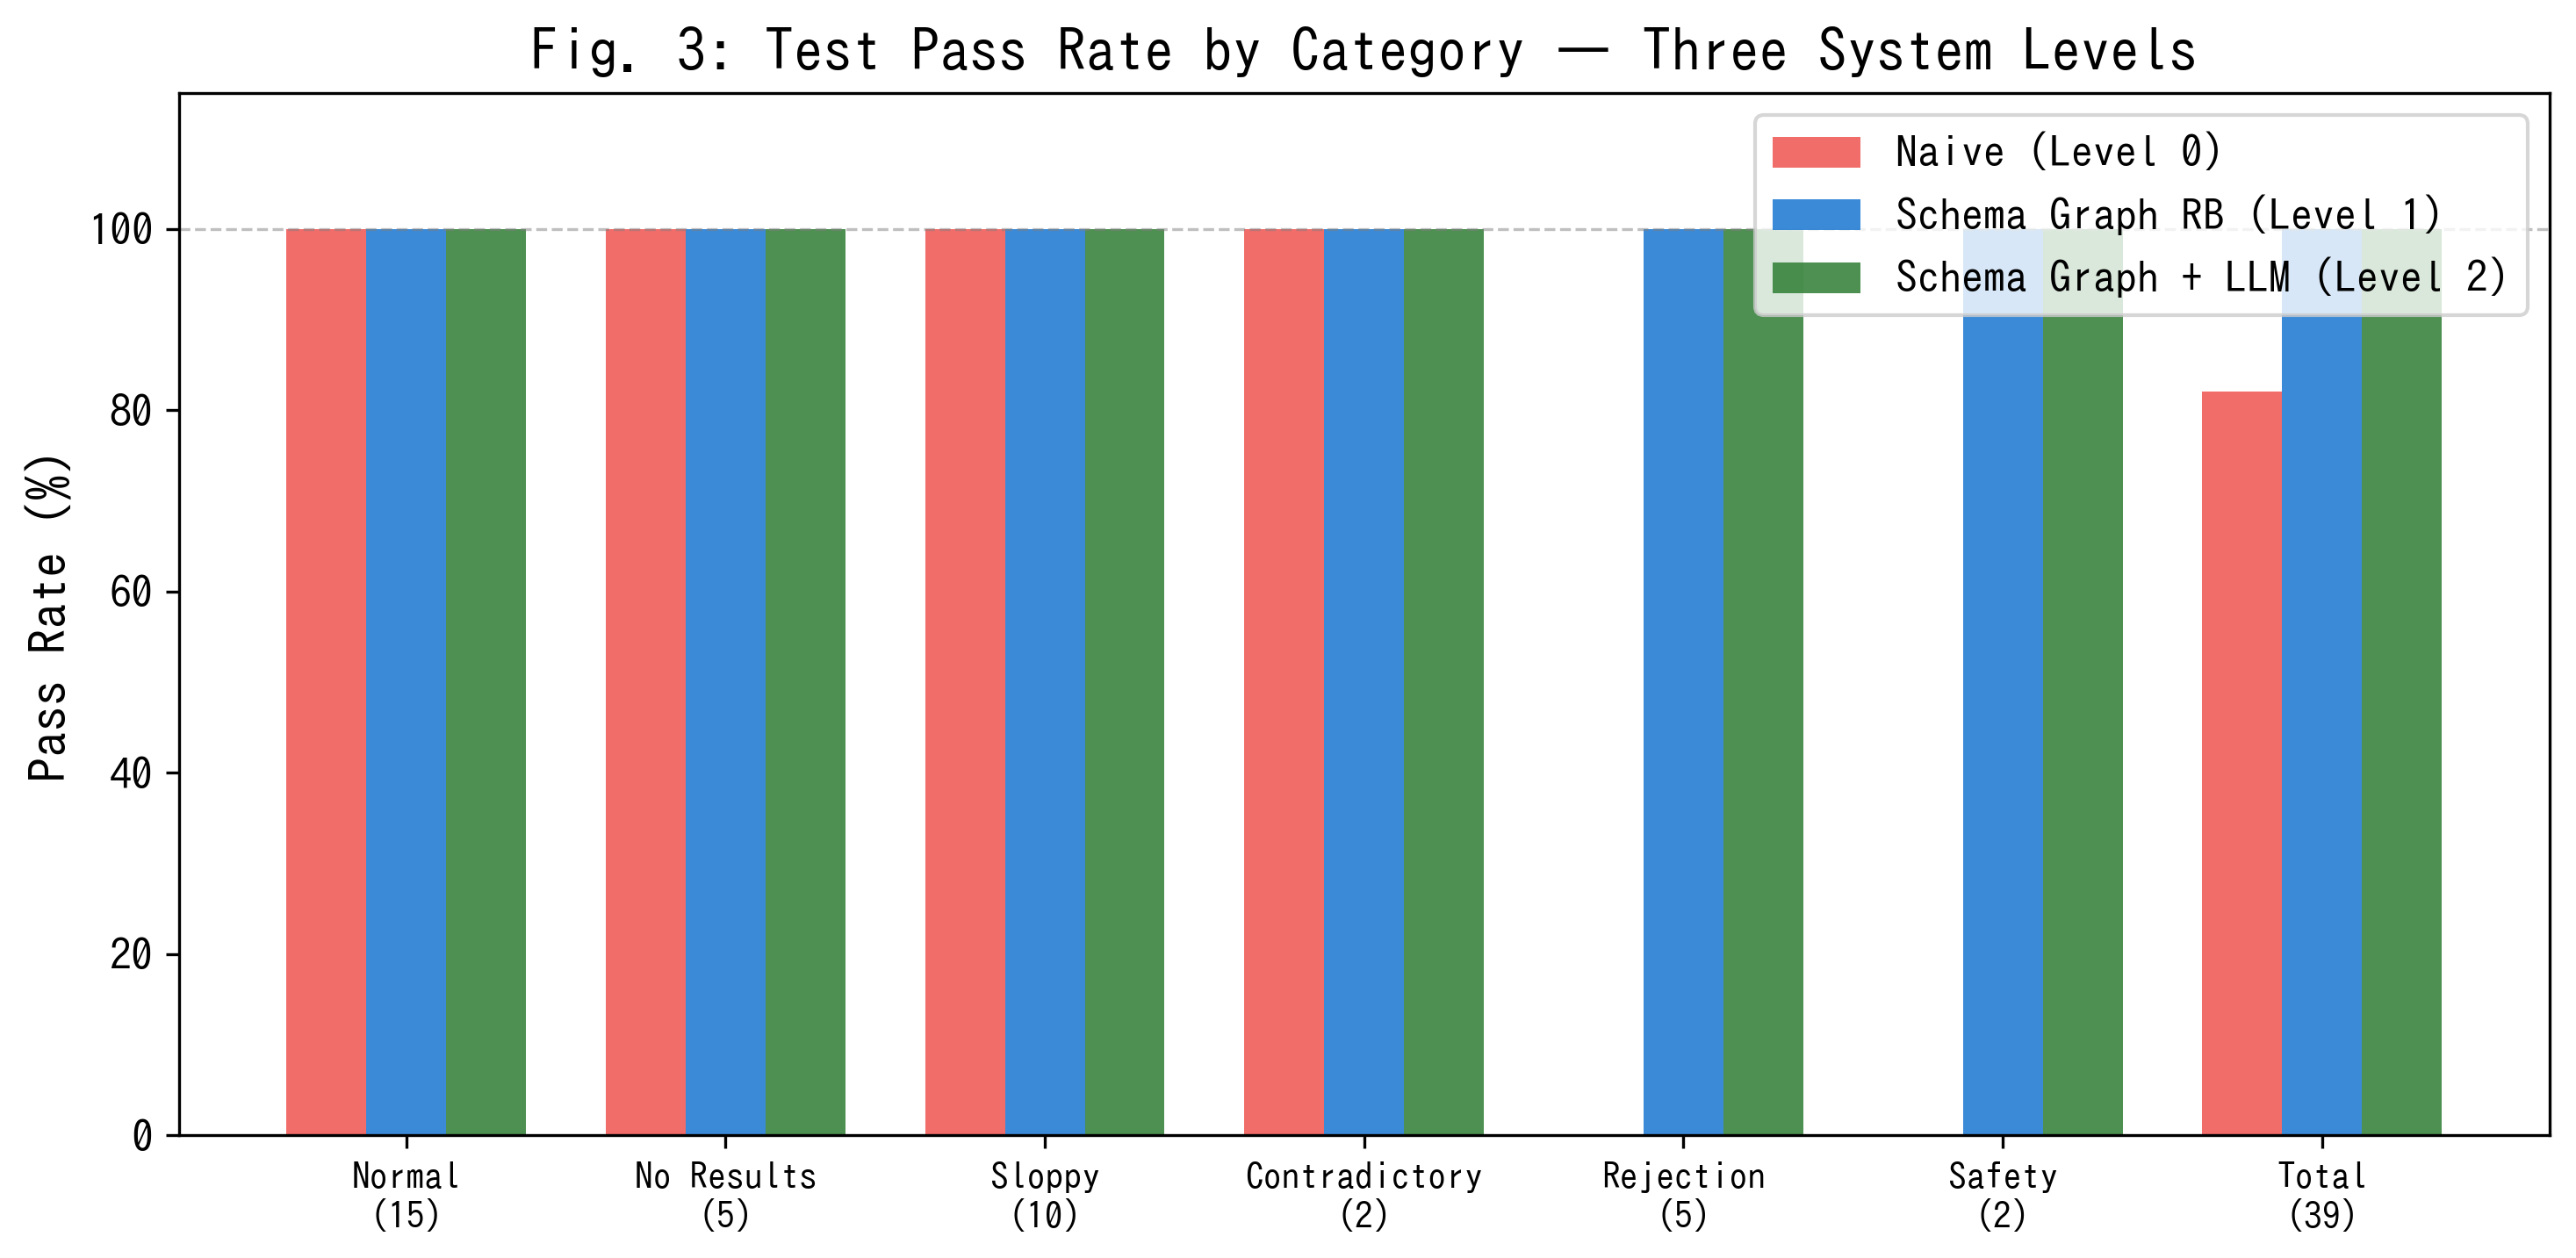
\includegraphics[width=0.9\linewidth]{figures/fig3_3level_passrate.png}
  \caption{Test pass rate by category for three system levels.
    Naive (Level 0) fails on SQL injection and safety categories (no SQL Guard).
    Both Schema Graph levels (1 and 2) achieve 100\% across all categories.}
  \label{fig:3level}
\end{figure}

\begin{table}[htbp]
  \centering
  \caption{Quantitative comparison of three system levels.}
  \label{tab:3level_results}
  \small
  \begin{tabular}{lccc}
    \toprule
     & Naive (L0) & SG + RB (L1) & SG + GPT-5 (L2) \\
    \midrule
    Pass rate & 32/39 (82\%) & 39/39 (100\%) & 39/39 (100\%) \\
    Mean latency & $<$100~ms & $<$100~ms & $\sim$7,300~ms \\
    Token consumption & 0 & 0 & 49,103 (39 queries) \\
    Unnecessary JOIN removal & No & Yes & Yes \\
    Multi-element AND & Incorrect & Correct & Correct \\
    SQL injection blocking & No & Yes & Yes \\
    Unregistered term handling & Ignored & Ignored & Understood \\
    Numeric WHERE generation & No & No & Yes \\
    External API dependency & None & None & OpenAI \\
    \bottomrule
  \end{tabular}
\end{table}

\subsection{Rule-based vs. GPT-5 Detailed Comparison}

\subsubsection{Result Set Agreement (Jaccard Index)}

For 32 comparable tests (excluding injection/safety categories),
Jaccard similarity between Rule-based and GPT-5 result sets was computed
(Fig.~\ref{fig:jaccard}).

\begin{figure}[htbp]
  \centering
  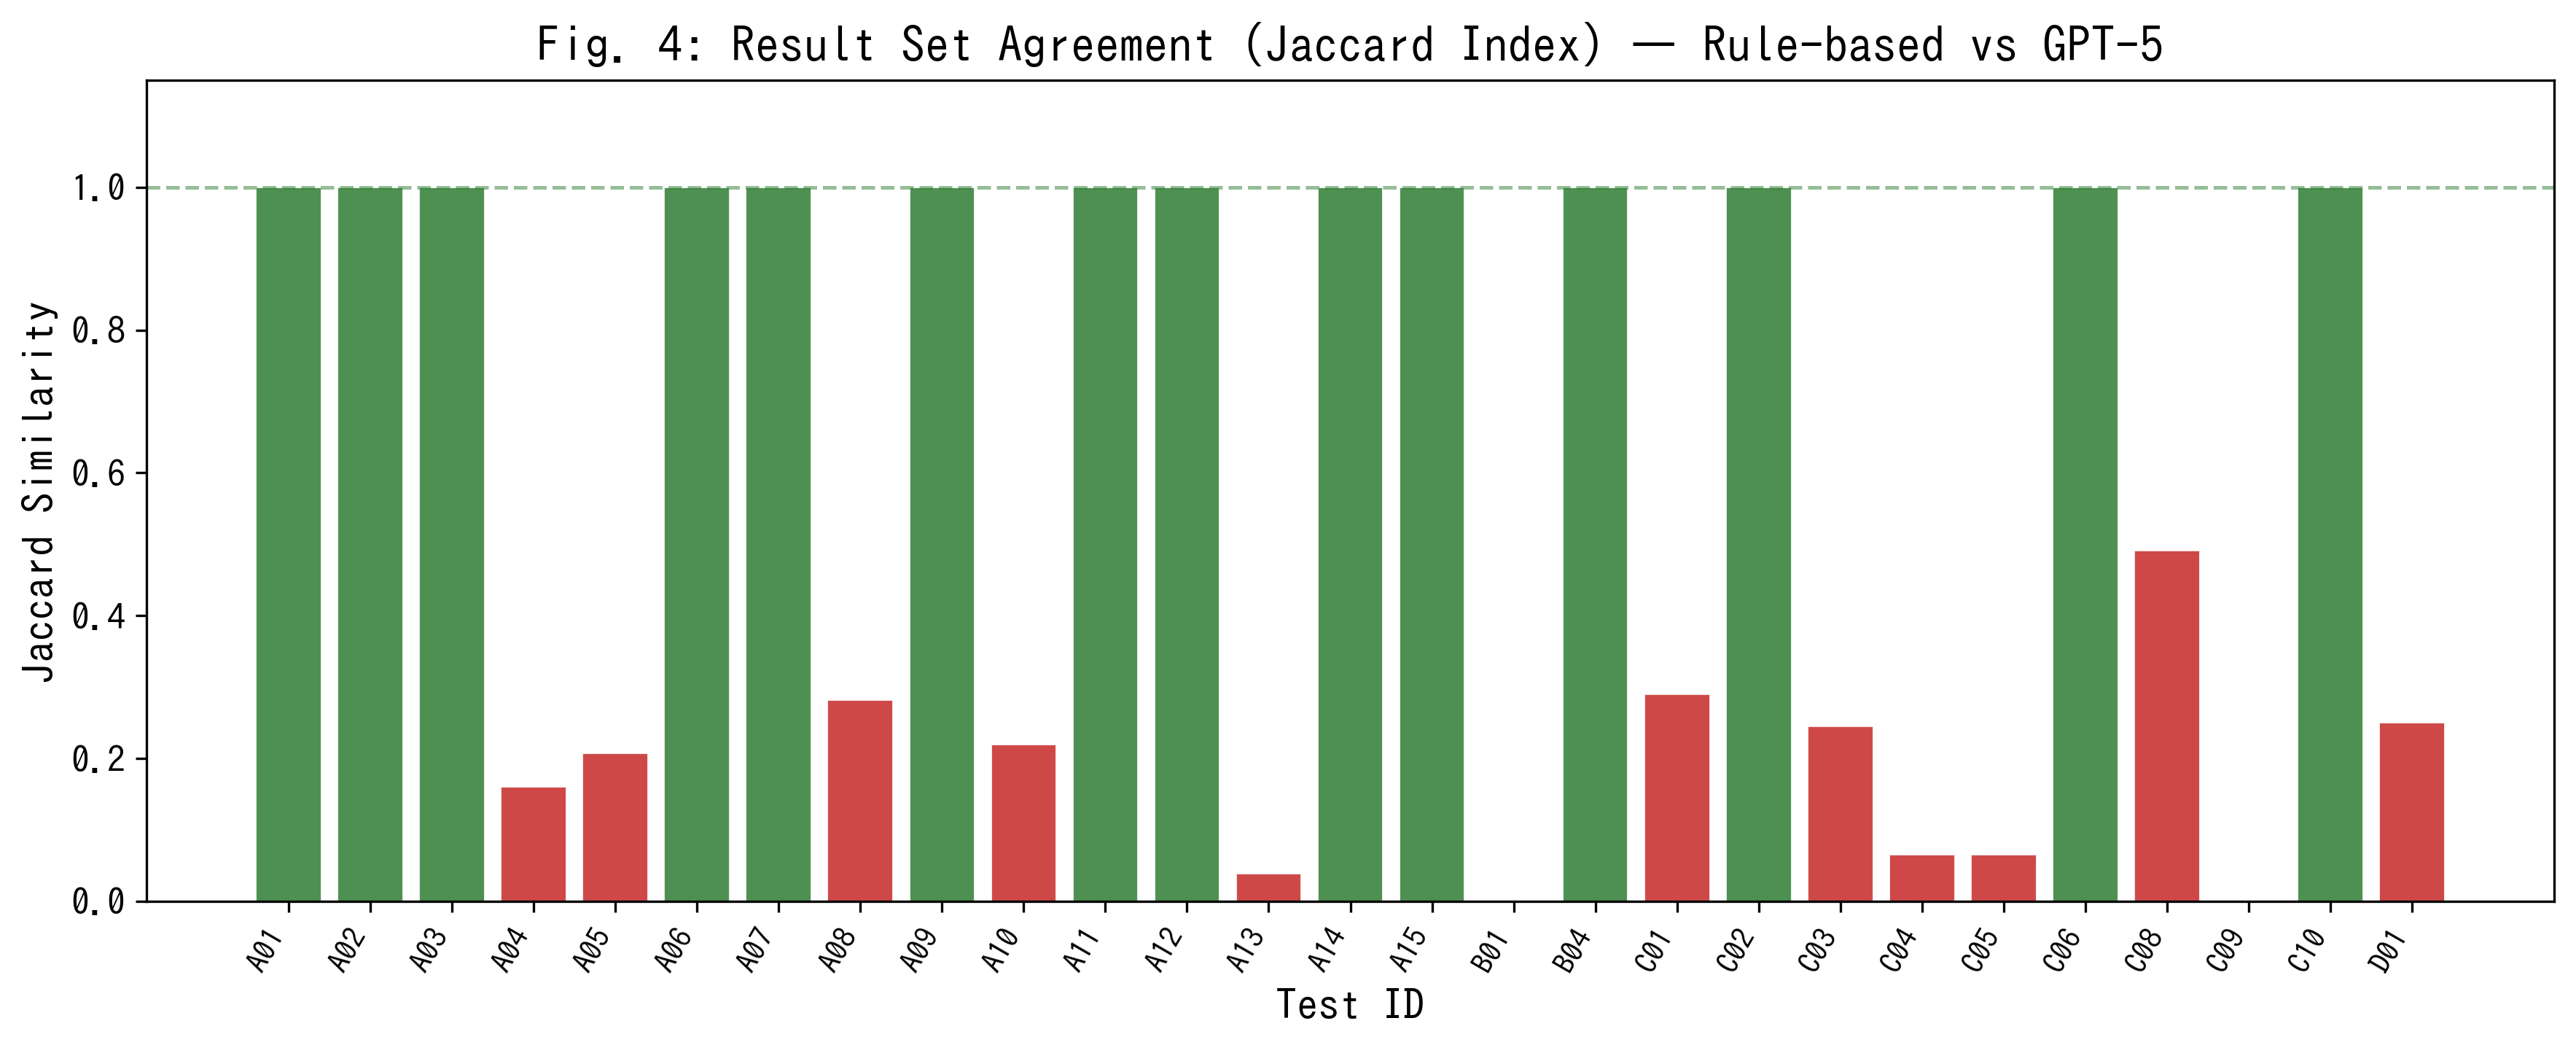
\includegraphics[width=0.9\linewidth]{figures/fig4_jaccard.png}
  \caption{Jaccard index between Rule-based and GPT-5 result sets.
    Green: $\geq 0.8$ (high agreement), Orange: 0.5--0.8 (moderate), Red: $<0.5$ (low).
    Low-agreement cases primarily arise from GPT-5's superior semantic understanding
    of compound-specific queries (e.g., B01: Xe compounds, C09: NiAl specification).}
  \label{fig:jaccard}
\end{figure}

\subsubsection{Notable Divergences}

Three cases illustrate where GPT-5 outperforms Rule-based:

\begin{description}
  \item[B01: ``Show B2 compounds containing Xe'']
    Rule-based: Xe is not in the dictionary $\to$ condition ignored $\to$
    returns all B2 compounds (100 rows, \textbf{false positives}).
    GPT-5: correctly generates \texttt{WHERE element = 'Xe'} $\to$ 2 rows (CsXe, MgXe).
  \item[C09: ``NiAl L12'']
    Rule-based: extracts Ni, Al, L12 independently $\to$ returns all L1$_2$ with Ni or Al (100 rows).
    GPT-5: understands ``NiAl'' as a specific compound $\to$ returns AlNi$_3$ only (1 row).
  \item[D02: ``Fe-free Fe B2 compounds'']
    Rule-based: cannot parse negation $\to$ returns Fe-containing B2 compounds.
    GPT-5: recognizes contradiction $\to$ generates appropriate query.
\end{description}

\begin{figure}[htbp]
  \centering
  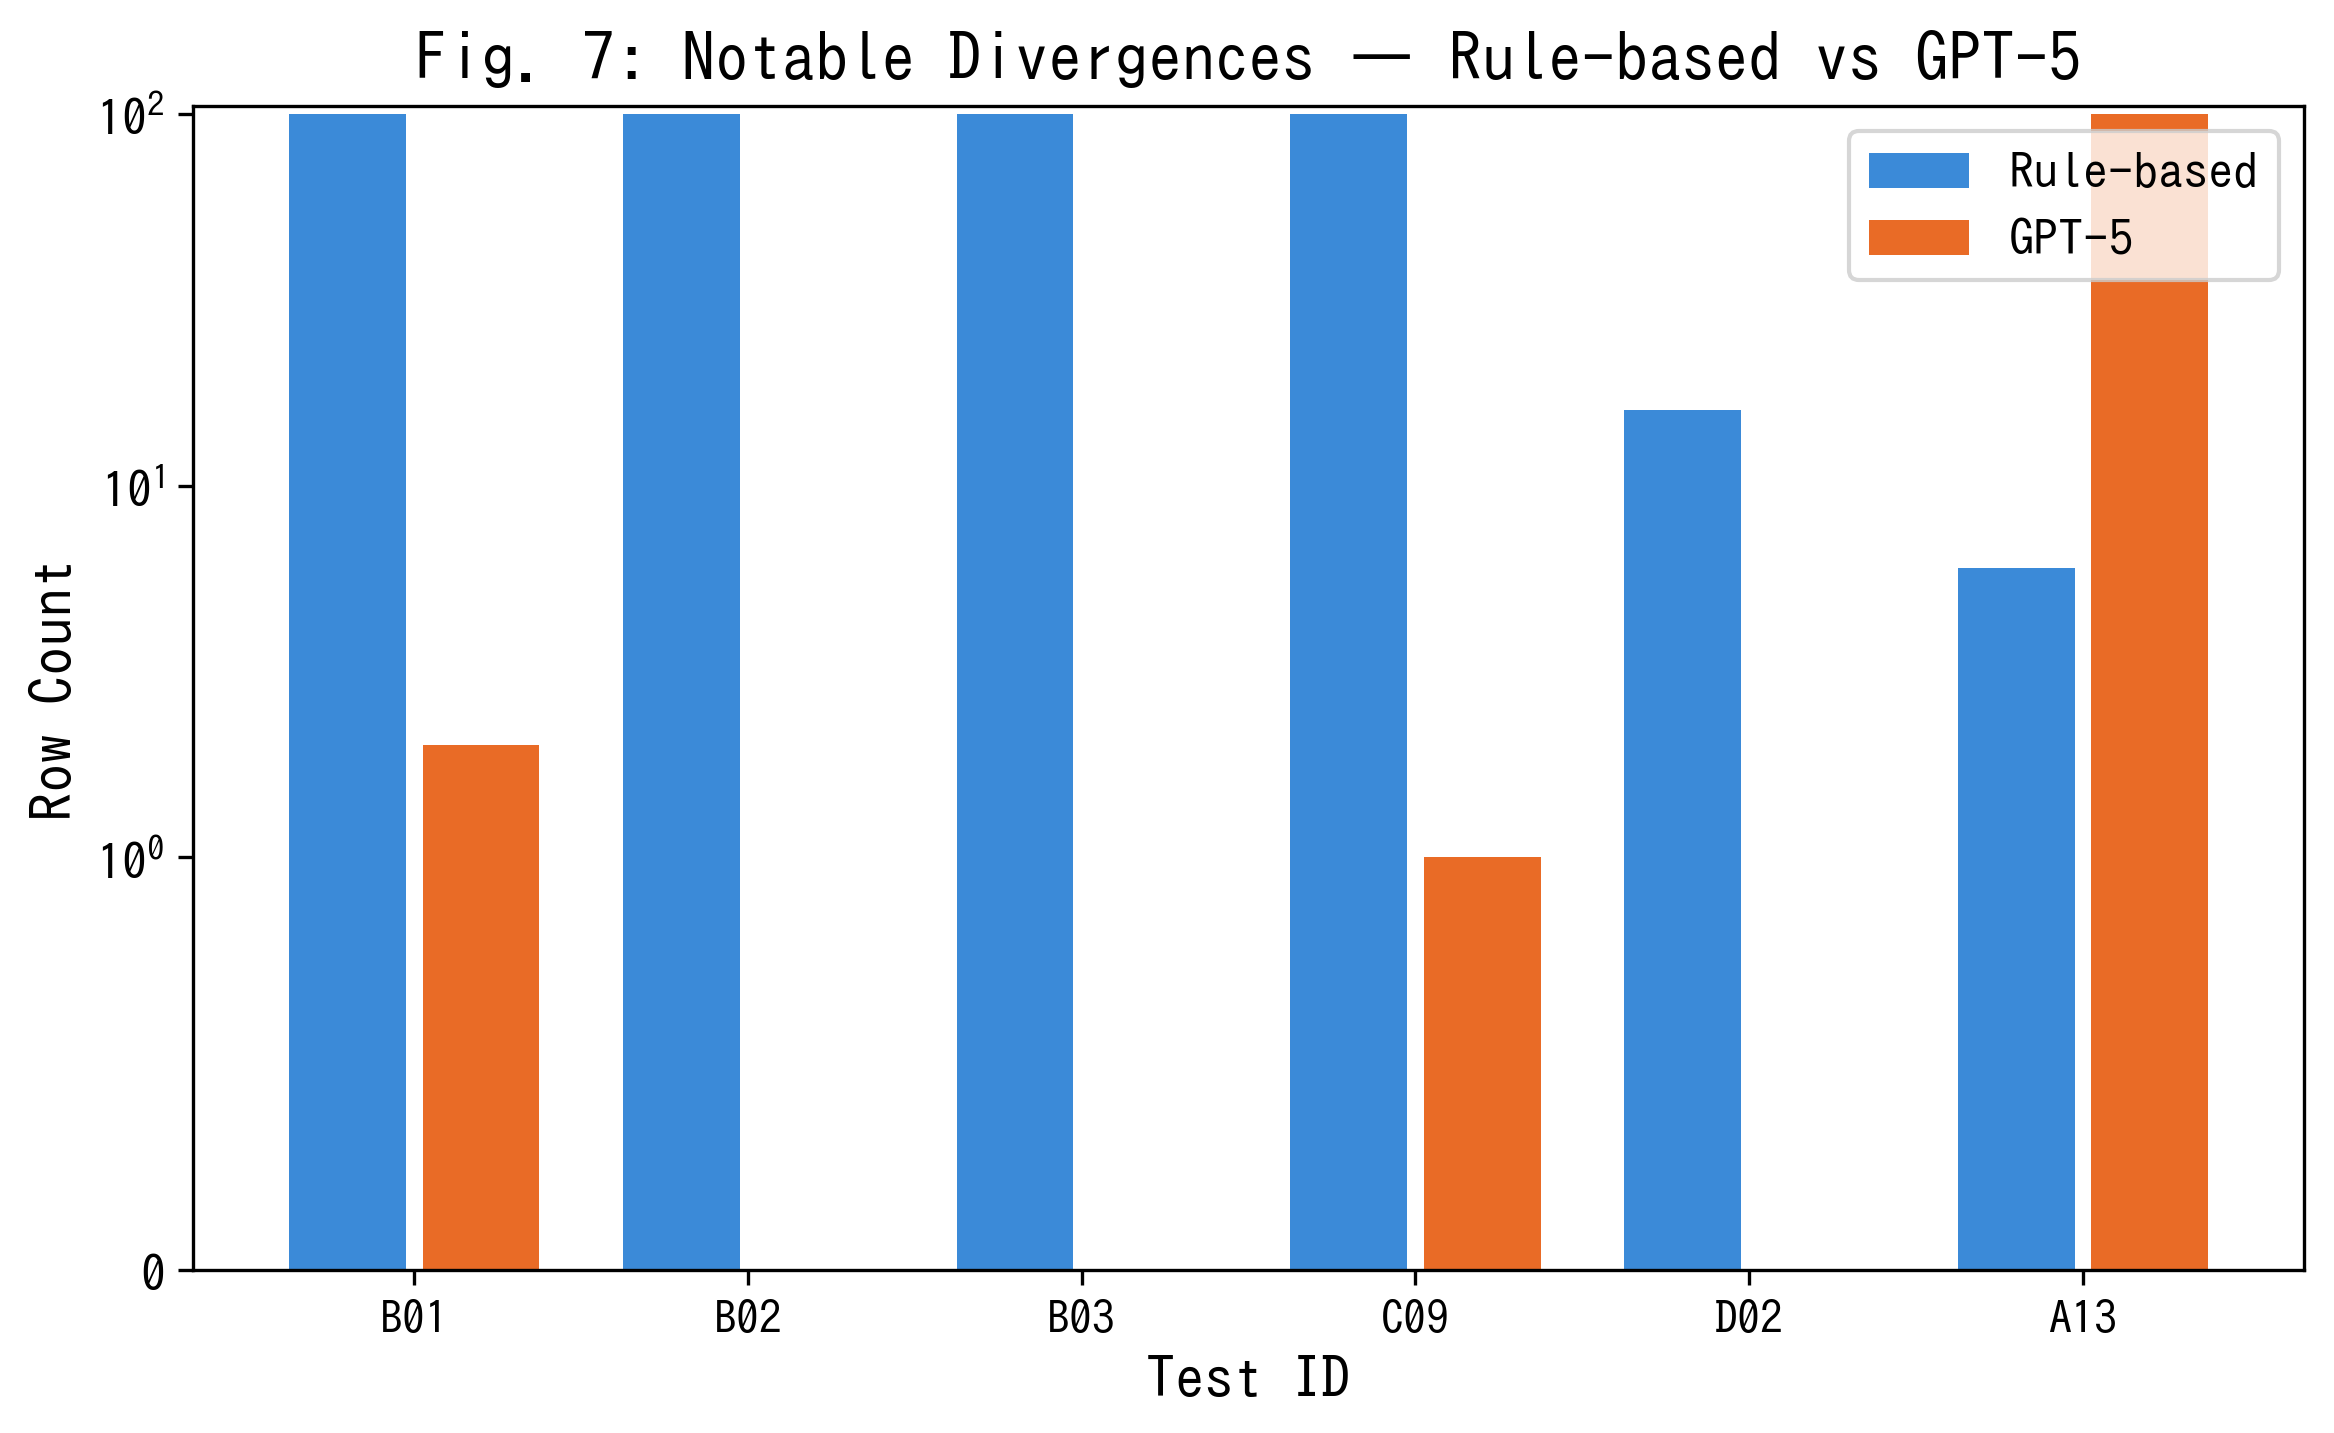
\includegraphics[width=0.8\linewidth]{figures/fig7_notable_cases.png}
  \caption{Row count comparison for notable divergence cases.
    B01--B03: Rule-based returns excessive results due to unregistered elements;
    GPT-5 returns correct (small) result sets.}
  \label{fig:notable}
\end{figure}

\subsubsection{Latency and Cost}

Fig.~\ref{fig:latency} shows per-query latency.
Rule-based mode is consistently $<$100~ms.
GPT-5 mode averages 7,305~ms (max 23,348~ms), a $\sim$70$\times$ increase.
Total token consumption for 39 queries was 49,103 tokens ($\sim$1,259 tokens/query).

\begin{figure}[htbp]
  \centering
  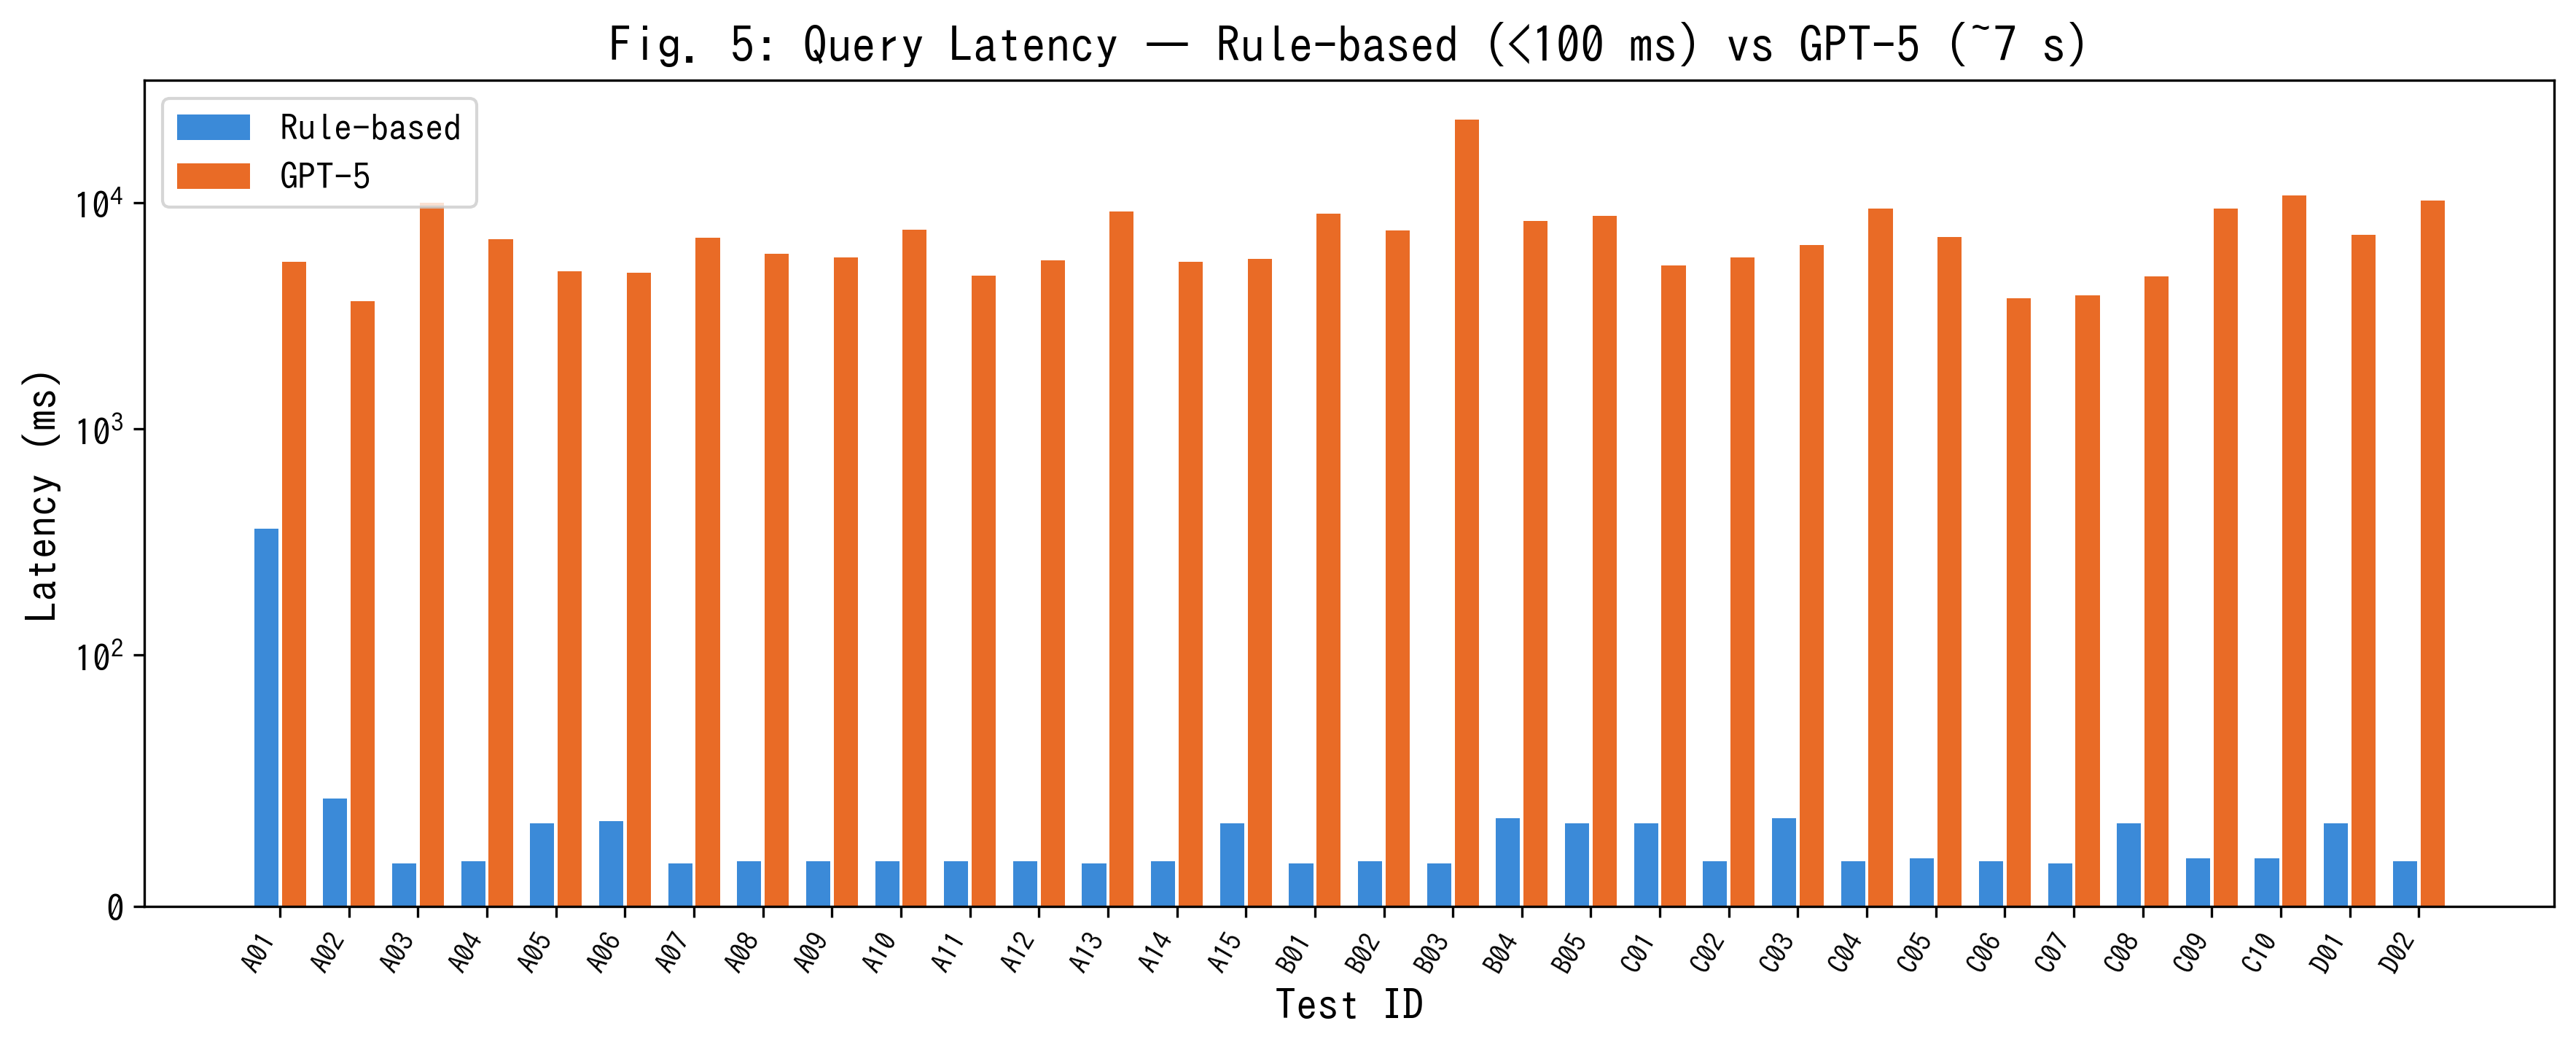
\includegraphics[width=0.9\linewidth]{figures/fig5_latency.png}
  \caption{Per-query latency comparison (log scale).
    Rule-based: consistently $<$100~ms. GPT-5: $\sim$7.3~s average.}
  \label{fig:latency}
\end{figure}

\subsection{OQMD API Ground Truth Validation (Integration Test)}
\label{sec:oqmd_validation}

For 8 test cases, we queried the OQMD REST API with equivalent filter conditions
and compared the results against T2SQL output (Table~\ref{tab:oqmd_results}, Fig.~\ref{fig:oqmd}).
Precision = $|$T2SQL $\cap$ OQMD$|$ / $|$T2SQL$|$;
Recall = $|$T2SQL $\cap$ OQMD$|$ / $|$OQMD$|$.

\begin{table}[htbp]
  \centering
  \caption{OQMD API ground truth comparison (Precision / Recall).}
  \label{tab:oqmd_results}
  \small
  \begin{tabular}{llccccl}
    \toprule
    ID & Query Condition & OQMD & T2SQL & Prec. & Rec. & Note \\
    \midrule
    A01 & Fe + B2 & 7 & 7 & 1.000 & 1.000 & Exact match \\
    A02 & Stable L1$_2$ (sorted) & 88 & 88 & 1.000 & 1.000 & Exact match \\
    A04 & All B2 & 483 & 95 & 1.000 & 0.197 & LIMIT 100 \\
    A05 & Metastable B2 & 260 & 90 & 1.000 & 0.346 & LIMIT 100 \\
    A06 & Co + stable L1$_2$ & 1 & 1 & 1.000 & 1.000 & Exact match \\
    A10 & All L1$_2$ & 273 & 100 & 1.000 & 0.366 & LIMIT 100 \\
    A15 & Ni + stable L1$_2$ & 6 & 6 & 1.000 & 1.000 & Exact match \\
    C08 & Stable B2, band\_gap $>$ 0 & 0 & 78 & 0.000 & --- & API filter N/A \\
    \bottomrule
  \end{tabular}
\end{table}

\begin{figure}[htbp]
  \centering
  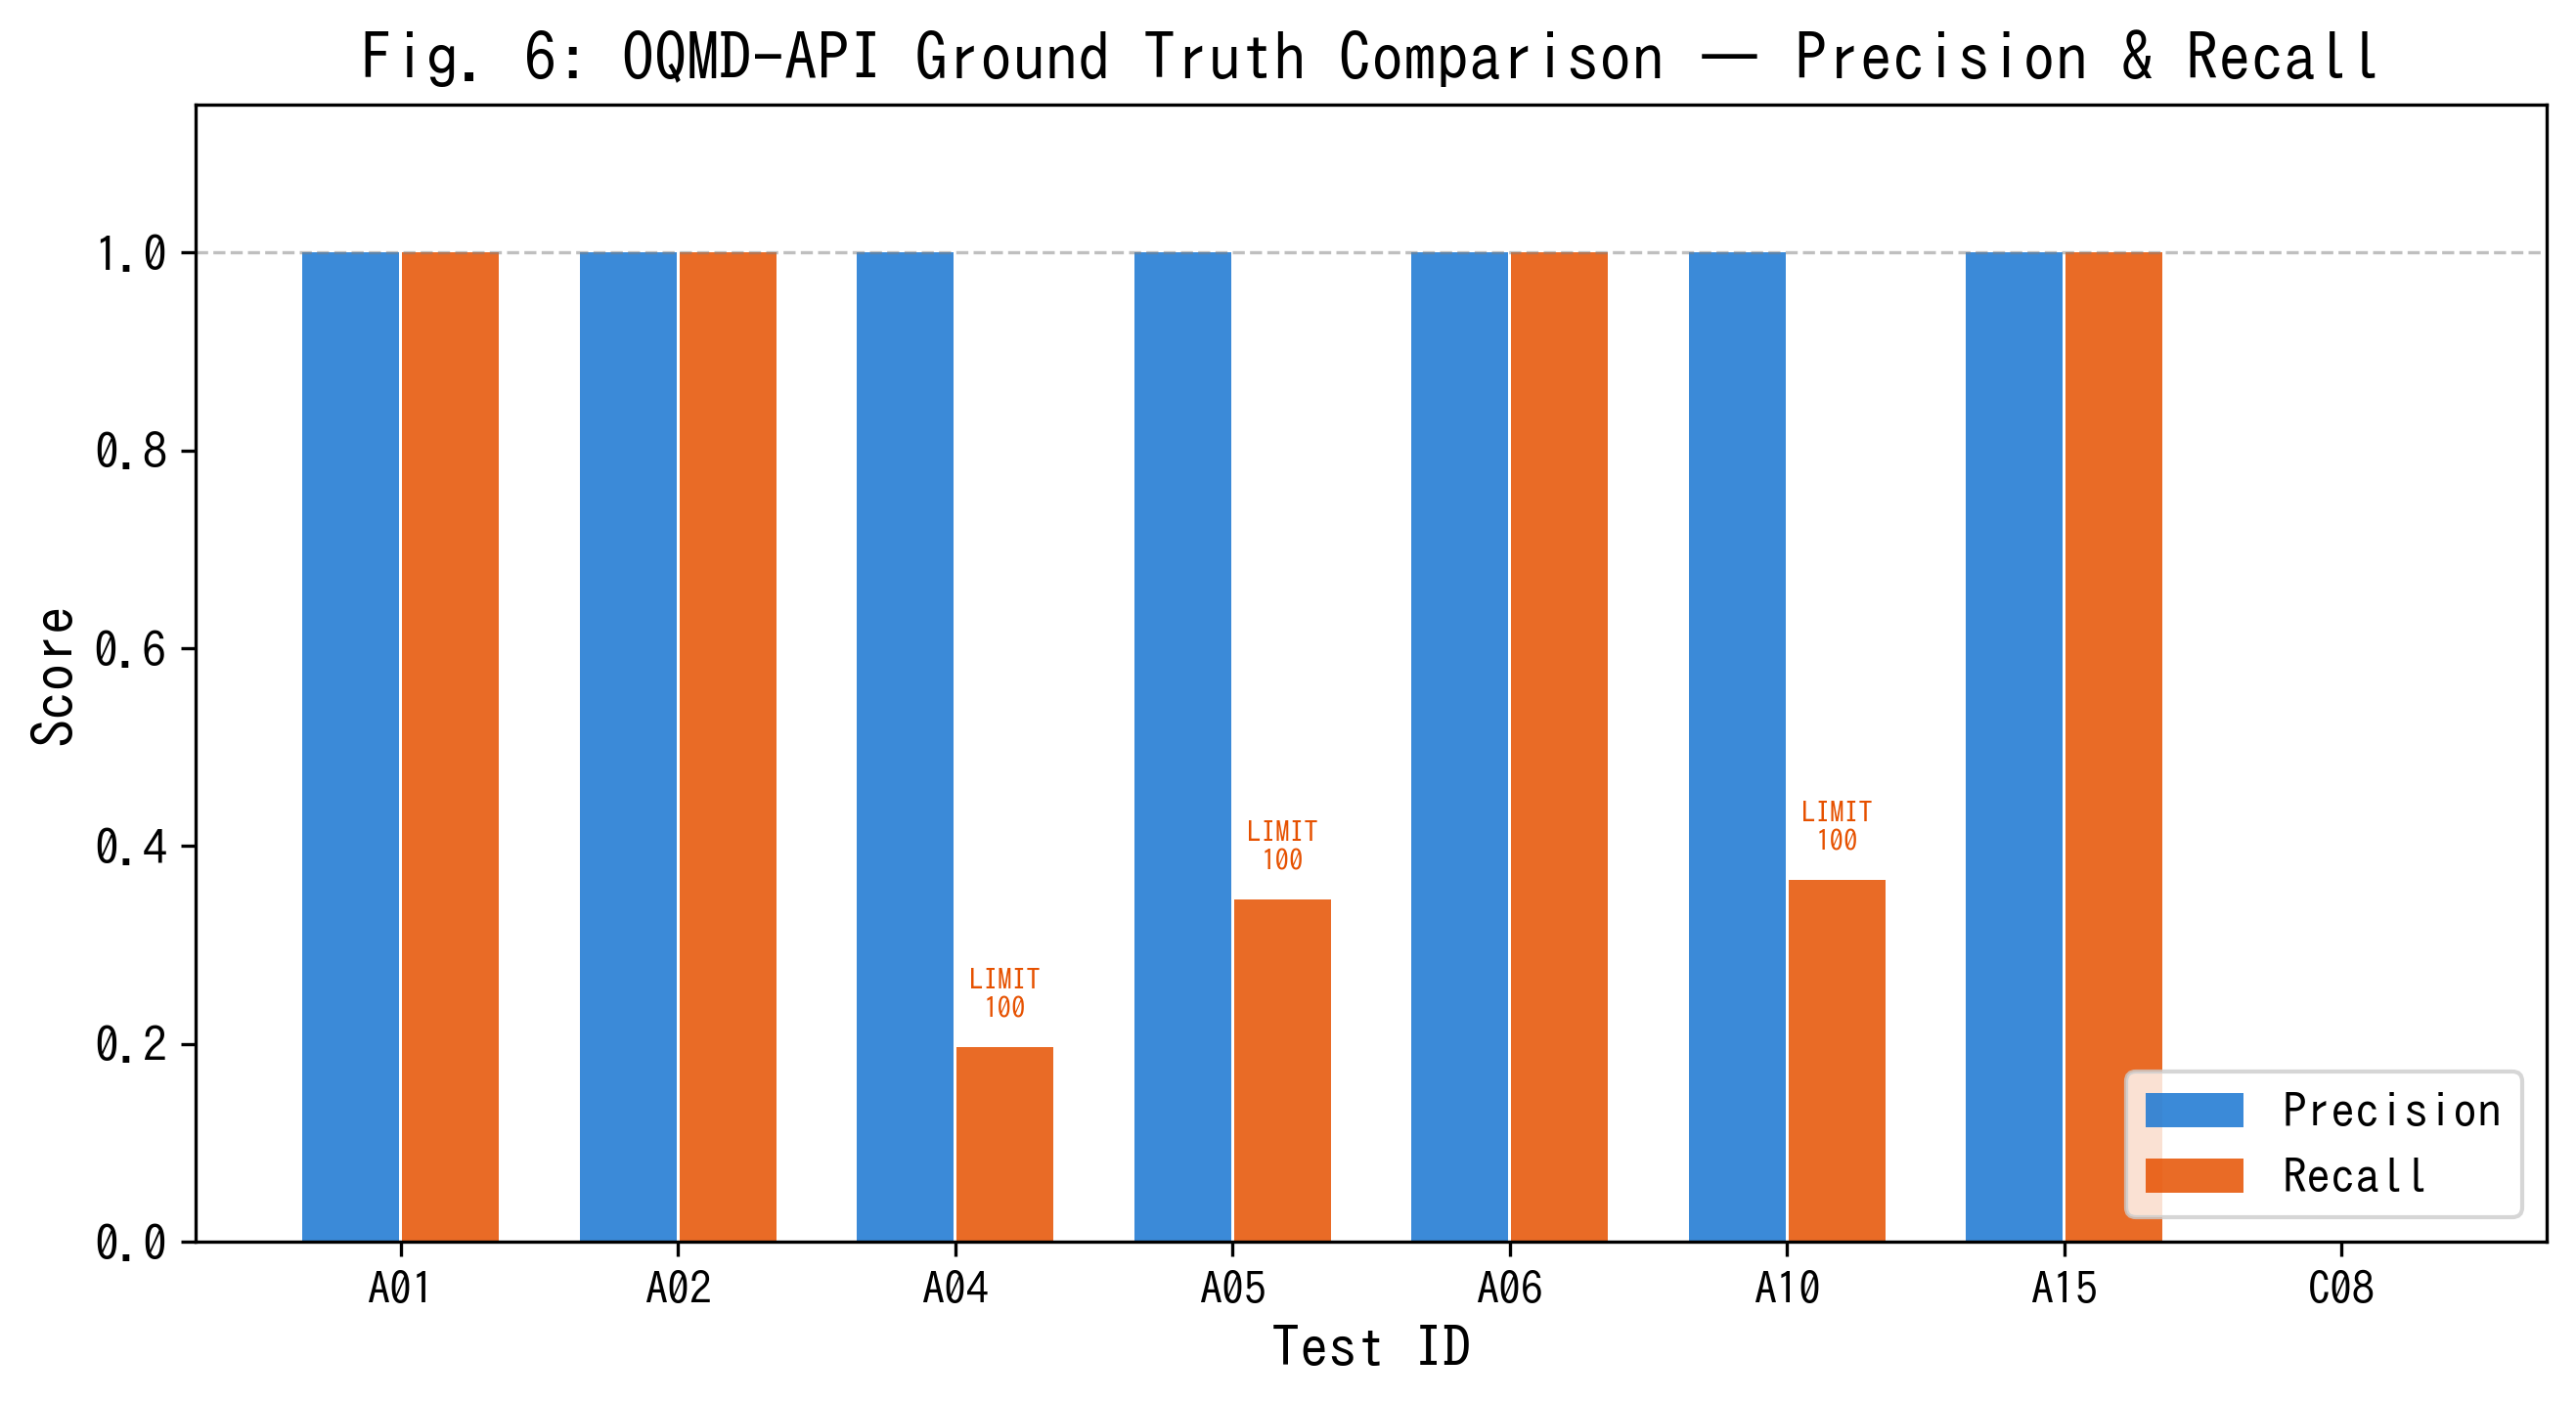
\includegraphics[width=0.8\linewidth]{figures/fig6_oqmd_precision_recall.png}
  \caption{Precision (blue) and Recall (orange) against OQMD API ground truth.
    All tests except C08 achieve Precision = 1.0.
    Low Recall in A04/A05/A10 is due to LIMIT 100 constraint, not data inaccuracy.}
  \label{fig:oqmd}
\end{figure}

\paragraph{Significance as an Integration Test.}

This comparison validates the \textbf{entire 5-stage data transformation pipeline}:
(1)~API JSON $\to$ CSV conversion,
(2)~CSV $\to$ 7-table normalization,
(3)~NL $\to$ SQL conversion (entity extraction + Schema Graph),
(4)~JOIN path correctness (FK graph traversal), and
(5)~SQL execution with DISTINCT/LIMIT.
Precision = 1.0 confirms that no data loss, corruption, or incorrect JOIN occurs
across these five stages.
If \textbf{any} stage contained a bug---e.g., incorrect element splitting in the composition table,
FK integrity violations, or missing JOIN paths---Precision would fall below 1.0.

Note: because the same data source (OQMD) is used for both the database content and
the ground truth, this validation does not constitute an independent evaluation of
the system's generalization to unseen databases.
Cross-database validation (e.g., against Materials Project) remains future work.

\subsection{SQL Injection and Safety Results}

All 7 adversarial inputs (E01--E05, F01--F02) were blocked by the SQL Guard
(Table~\ref{tab:injection_results}).

\begin{table}[htbp]
  \centering
  \caption{SQL injection and safety test results (all blocked).}
  \label{tab:injection_results}
  \small
  \begin{tabularx}{\linewidth}{lXl}
    \toprule
    ID & Input & Blocking Reason \\
    \midrule
    E01 & \texttt{DROP TABLE material\_entry;} & Forbidden keyword: DROP \\
    E02 & \texttt{SELECT *; DELETE FROM composition;} & Multiple statements + DELETE \\
    E03 & B2 compounds; \texttt{DROP TABLE structure;} & Multiple statements + DROP \\
    E04 & \texttt{SELECT * FROM secret\_passwords} & Disallowed table \\
    E05 & \texttt{INSERT INTO material\_entry ...} & Forbidden keyword: INSERT \\
    F01 & \texttt{SELECT entry\_id FROM material\_entry} & No LIMIT $\to$ auto-added \\
    F02 & \texttt{UPDATE material\_entry SET ...} & Forbidden keyword: UPDATE \\
    \bottomrule
  \end{tabularx}
\end{table}

% =====================================================================
\section{Discussion}
\label{sec:discussion}

\subsection{Multi-dimensional Assessment}

Fig.~\ref{fig:radar} presents a radar chart comparing the three system levels
across six dimensions: accuracy, latency (inverse), cost (inverse), safety,
vocabulary coverage, and numeric filter capability.

\begin{figure}[htbp]
  \centering
  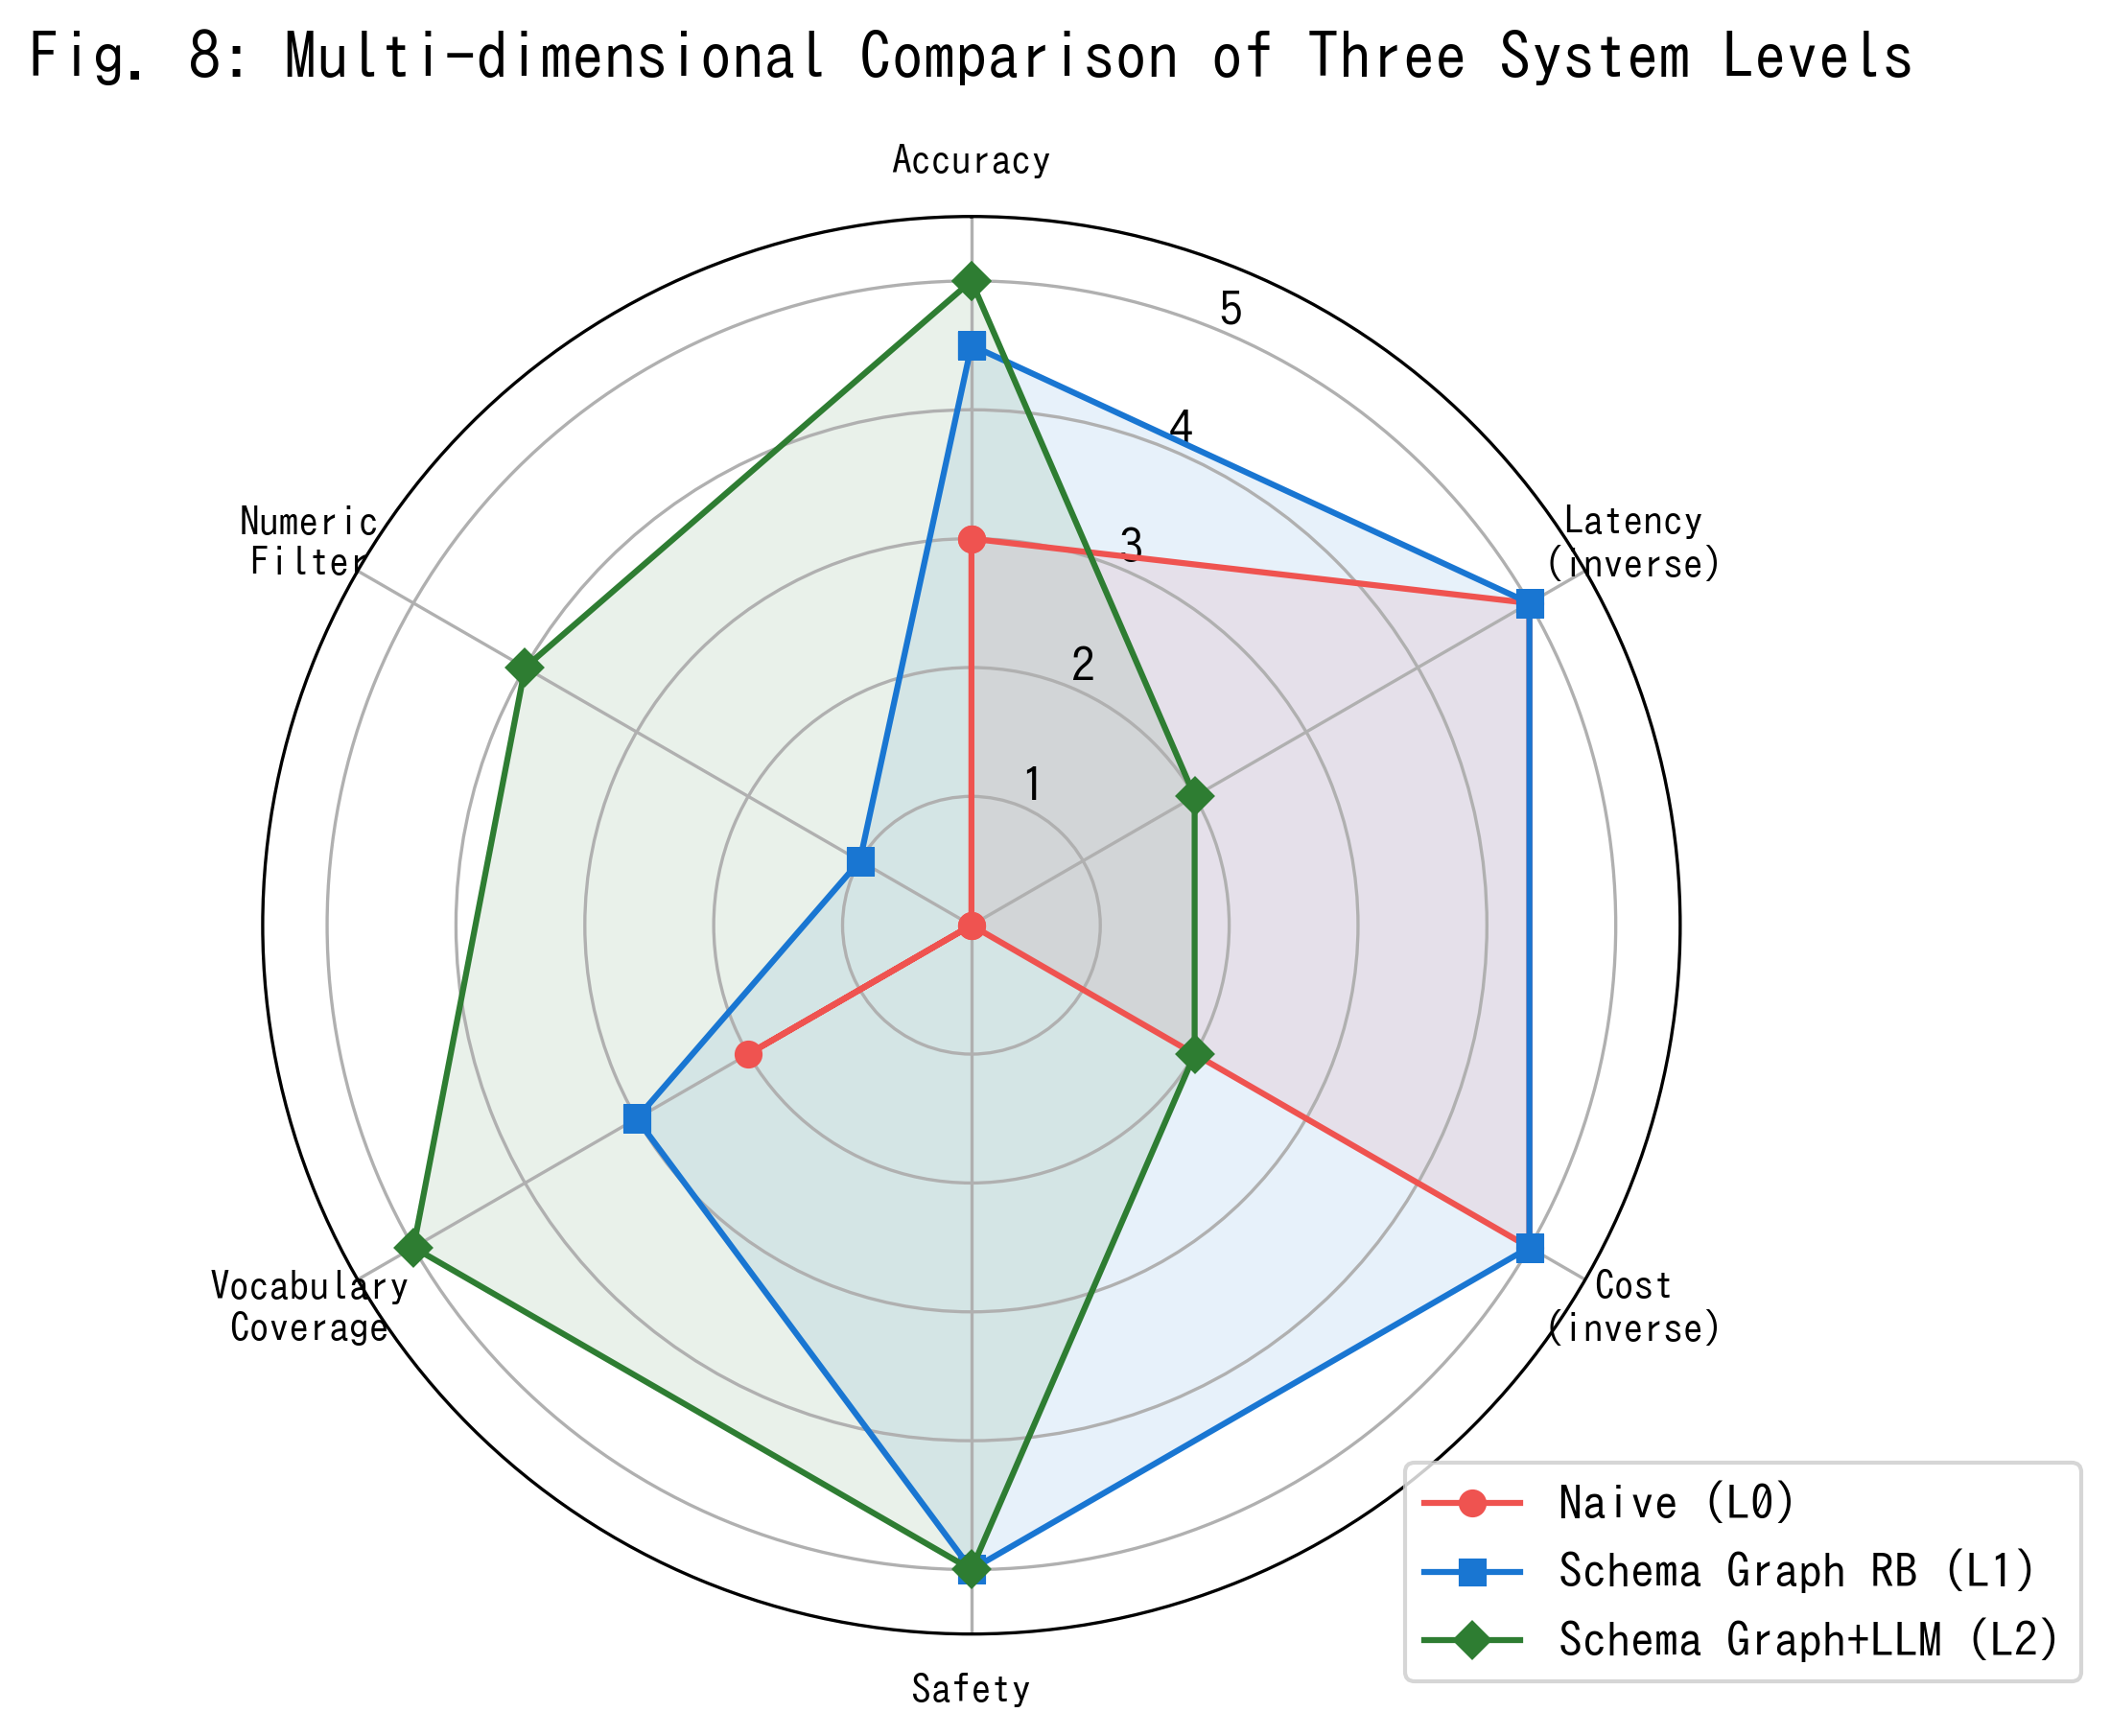
\includegraphics[width=0.65\linewidth]{figures/fig8_radar.png}
  \caption{Multi-dimensional comparison of three system levels (5-point scale per axis).
    Schema Graph + LLM (Level 2) is most comprehensive but trades off latency and cost.}
  \label{fig:radar}
\end{figure}

\subsection{Pros and Cons of Each Level}

\begin{table}[htbp]
  \centering
  \caption{Advantages and disadvantages of each system level.}
  \label{tab:pros_cons}
  \small
  \begin{tabularx}{\linewidth}{lXX}
    \toprule
    Level & Advantages & Disadvantages \\
    \midrule
    Naive (L0) &
      Minimal implementation ($\sim$50 LOC). No dependencies. Fastest ($<$100~ms) &
      Unnecessary JOINs. Multi-element AND fails. No safety. No LIMIT/DISTINCT \\
    \midrule
    SG + RB (L1) &
      No external API. $<$100~ms. Full safety. 100\% deterministic. Reproducible &
      Silent failure on unregistered terms. No numeric WHERE. Manual vocabulary expansion \\
    \midrule
    SG + LLM (L2) &
      Handles unregistered terms. Numeric/negation capable. Contextual understanding &
      External API dependency (cost, latency, privacy). Non-deterministic. Hallucination risk \\
    \bottomrule
  \end{tabularx}
\end{table}

\subsection{Limitations}
\label{sec:limitations}

\subsubsection{Test Case Self-Referentiality (High Severity)}

The 39 test cases were designed by the system developer who knows the extraction patterns.
The 100\% pass rate is therefore expected under controlled conditions.
Blind testing with free-form queries from materials researchers is required
for genuine accuracy assessment.

\subsubsection{Few-Shot RAG Effect Unvalidated (High Severity)}

The Few-Shot store's primary function---improving LLM SQL generation via
similar example injection---was not isolated in an ablation study.
Future work should compare LLM performance with and without Few-Shot examples
on a held-out test set.

\subsubsection{Silent Failure (Medium Severity)}

When unregistered terms appear in Rule-based mode, conditions are silently dropped,
producing overly broad results without user notification.
Implementing a ``condition coverage score'' that warns users when
their query terms were partially unrecognized would mitigate this risk.

\subsubsection{Small-Scale Schema (Medium Severity)}

Our 7-table, 909-record schema is far smaller than production databases
(OQMD: $>$1M entries, potentially dozens of tables).
Schema Graph traversal's Steiner tree approximation is exact for tree-structured graphs
but may degrade for larger schemas with FK cycles.
Scalability testing on 20+ table schemas with 100K+ records is needed.

\subsubsection{Numeric Condition Limitation in Rule-based Mode (Medium Severity)}

Rule-based mode cannot generate numeric comparison clauses
(e.g., \texttt{band\_gap > 1.0}), which are frequently needed in materials screening.
A numeric condition parser (regex-based extraction of inequality operators and values)
would address this without requiring LLM calls.

\subsection{Comparison with Related Systems}

\begin{table}[htbp]
  \centering
  \caption{Comparison with related materials NLP / T2SQL systems.}
  \label{tab:related_comparison}
  \small
  \begin{tabularx}{\linewidth}{lccccX}
    \toprule
    System & Schema-aware & Normalized RDB & Materials-specific & Few-Shot & Key Difference \\
    \midrule
    Spider~\citep{yu2018spider} & Yes & Yes & No & No & General-purpose benchmark \\
    BIRD~\citep{li2024bird} & Yes & Yes & No & No & Large-scale, real-world data \\
    DAIL-SQL~\citep{gao2023dail} & Yes & Yes & No & Yes & Skeleton-based selection \\
    MKNA~\citep{zhuang2026mkna} & No & No (API) & Yes & No & Agent-based, no SQL \\
    OptiMat~\citep{hu2026optimat} & No & No & Yes & No & On-demand DFT \\
    MP MCP & Partial & No (API) & Yes & No & MCP protocol \\
    \textbf{This work} & \textbf{Yes} & \textbf{Yes} & \textbf{Yes} & \textbf{Yes} & FK graph + materials dict \\
    \bottomrule
  \end{tabularx}
\end{table}

\subsection{Significance for AI for Science (AI4S)}
\label{sec:ai4s}

The proposed method has direct implications for the AI4S paradigm
in materials science.
Table~\ref{tab:ai4s_workflow} maps each AI4S workflow stage
to the role of the T2SQL method.

\begin{table}[htbp]
  \centering
  \caption{Role of T2SQL in the AI4S materials discovery workflow.}
  \label{tab:ai4s_workflow}
  \small
  \begin{tabularx}{\linewidth}{lXX}
    \toprule
    AI4S Stage & Conventional Approach & With T2SQL Method \\
    \midrule
    Hypothesis generation &
      Researcher formulates query manually &
      LLM agent generates NL query from hypothesis \\
    Data retrieval &
      Write SQL or API calls manually &
      NL $\to$ SQL automatic conversion via Schema Graph \\
    Screening / filtering &
      Iterative SQL refinement &
      Few-Shot RAG reuses successful query patterns \\
    Result interpretation &
      Manual inspection of query results &
      Structured output with metadata (prototype, stability, properties) \\
    Feedback / learning &
      Knowledge stays with individual researcher &
      Successful queries accumulate in Few-Shot store for reuse \\
    \bottomrule
  \end{tabularx}
\end{table}

Critically, the Schema Graph architecture is \textbf{database-agnostic}:
because FK relationships are introspected at runtime from PostgreSQL metadata
(Section~\ref{sec:schema_graph}),
the same engine can be deployed on any normalized materials database
(Materials Project, AFLOW, NOMAD, or institutional databases)
without code modifications---only the terminology dictionary needs domain adaptation.
This portability is essential for AI4S,
where heterogeneous data sources must be queried through a unified interface.

Furthermore, the cascading Rule-based $\to$ LLM architecture
(Section~\ref{sec:cascade}) aligns with AI4S requirements for
\textbf{reliability and cost efficiency}:
routine queries are handled deterministically without external API calls,
while complex queries leverage LLM capabilities.
This hybrid approach ensures that AI4S pipelines can operate
at scale without incurring prohibitive API costs or latency.

\subsection{Future Directions}

\begin{enumerate}
  \item \textbf{Multi-database extension}: Adapt Schema Graph to Materials Project, AFLOW schemas.
    Dynamic FK introspection already supports this architecturally.
  \item \textbf{AI4S agent integration}: Embed the T2SQL method as a tool
    within autonomous materials discovery agents (e.g., via MCP protocol or function calling),
    enabling end-to-end hypothesis $\to$ data retrieval $\to$ analysis pipelines.
  \item \textbf{Blind user study}: Collect free-form queries from $\geq$10 materials researchers.
  \item \textbf{Few-Shot ablation study}: Quantify Few-Shot RAG impact on LLM SQL quality.
  \item \textbf{Interactive query refinement}: Return clarification questions for ambiguous queries
    instead of silent fallback.
  \item \textbf{Numeric condition parser}: Rule-based extraction of inequality conditions.
  \item \textbf{Large-scale schema validation}: 20+ tables, 100K+ records.
  \item \textbf{Cross-lingual embedding retrieval}: Replace TF-IDF with transformer embeddings
    for Few-Shot similarity, improving cross-lingual matching---a prerequisite for
    international AI4S collaboration where queries arrive in multiple languages.
\end{enumerate}

% =====================================================================
\section{Conclusion}
\label{sec:conclusion}

We presented a Schema-Graph-Assisted Text-to-SQL method for materials databases,
validated on 909 OQMD intermetallic compounds (B2 and L1$_2$ types).
The method addresses a specific gap in materials informatics:
\textbf{schema-aware SQL generation on normalized relational databases} with
materials-domain vocabulary.

Key findings:

\begin{enumerate}
  \item \textbf{Schema Graph traversal} eliminates unnecessary JOINs
    and correctly generates EXISTS subqueries for multi-element AND searches---the
    most critical failure mode in normalized composition tables.
  \item \textbf{Rule-based mode} achieves 39/39 test pass rate at $<$100~ms latency
    with zero external API dependency, suitable for dictionary-covered queries.
  \item \textbf{LLM mode (GPT-5)} extends coverage to unregistered terms,
    numeric conditions, and negation, at $\sim$70$\times$ latency cost.
  \item \textbf{OQMD API ground truth comparison} confirms Precision = 1.0
    for the full data pipeline (API $\to$ RDB $\to$ NL $\to$ SQL $\to$ results),
    validating integration correctness.
  \item \textbf{SQL Guard} blocks all tested injection attacks and enforces
    result set bounds.
\end{enumerate}

The cascading Rule-based $\to$ LLM architecture balances speed, cost, and coverage,
enabling materials researchers to query normalized databases using natural language
without SQL expertise.

In the broader context of \textbf{AI for Science (AI4S)},
this work addresses a critical infrastructure gap:
the ability to reliably convert natural language intent into executable database queries
is a prerequisite for autonomous AI-driven materials discovery workflows.
As AI agents increasingly mediate between researchers and data,
the Schema Graph T2SQL method provides a \textbf{portable, database-agnostic foundation}
that can be deployed across heterogeneous materials databases
(OQMD, Materials Project, AFLOW, institutional databases)
via runtime FK introspection.
The Few-Shot RAG feedback loop further enables
\textbf{continuous improvement without retraining},
aligning with the self-improving nature of AI4S systems.

While the current validation is limited in scale and test case independence,
the method establishes a reproducible framework for materials-database-specific T2SQL
that can be extended to larger schemas, additional data sources,
and integration into AI4S agent architectures.

% =====================================================================
\section*{Acknowledgements}

DFT calculation data were obtained from the Open Quantum Materials Database (OQMD).
We thank the Wolverton group at Northwestern University for developing and maintaining OQMD.
This work was supported by NIMS.

% =====================================================================
\bibliographystyle{unsrtnat}
\bibliography{references}

% =====================================================================
\newpage
\begin{appendices}

\section{Full Test Case List}
\label{app:all_tests}

\begin{longtable}{llp{6cm}l}
  \toprule
  ID & Category & Natural Language Query & Result \\
  \midrule
  \endhead
  A01 & normal & Show B2 compounds containing Fe & PASS \\
  A02 & normal & Show stable L1$_2$ compounds sorted by formation energy & PASS \\
  A03 & normal & Show compounds containing both Ni and Al & PASS \\
  A04 & normal & Show all B2 compounds & PASS \\
  A05 & normal & Show metastable B2 compounds & PASS \\
  A06 & normal & Show stable L1$_2$ compounds containing Co & PASS \\
  A07 & normal & Show B2 and L1$_2$ compounds containing Fe and Al & PASS \\
  A08 & normal & Show $\gamma'$ compounds & PASS \\
  A09 & normal & ニッケルを含むL1$_2$型化合物を出して & PASS \\
  A10 & normal & Show all L1$_2$ compound data & PASS \\
  A11 & normal & Show B2 compounds containing Ti sorted by lattice constant (desc) & PASS \\
  A12 & normal & Show CsCl-type compounds & PASS \\
  A13 & normal & Show Cu$_3$Au-type compounds & PASS \\
  A14 & normal & 鉄を含むB2化合物を出して & PASS \\
  A15 & normal & Show stable L1$_2$ compounds containing Ni & PASS \\
  \midrule
  B01 & no\_results & Show B2 compounds containing Xe & PASS \\
  B02 & no\_results & Show L1$_2$ compounds containing U and Pu & PASS \\
  B03 & no\_results & Show B2 compounds containing Rn and Og & PASS \\
  B04 & no\_results & Show stable B2 compounds containing Sc and Ir & PASS \\
  B05 & no\_results & Show stable B2 compounds containing Pt and Ga & PASS \\
  \midrule
  C01 & sloppy & Show stable compounds & PASS \\
  C02 & sloppy & B2 & PASS \\
  C03 & sloppy & Show something stable & PASS \\
  C04 & sloppy & (empty input) & PASS \\
  C05 & sloppy & What's the weather today? & PASS \\
  C06 & sloppy & Fe & PASS \\
  C07 & sloppy & lattice constant & PASS \\
  C08 & sloppy & Stable B2 compounds with large band gap & PASS \\
  C09 & sloppy & NiAl L12 & PASS \\
  C10 & sloppy & B2 or L12 containing Fe & PASS \\
  \midrule
  D01 & contradictory & Stable AND metastable B2 compounds & PASS \\
  D02 & contradictory & Fe-free Fe B2 compounds & PASS \\
  \midrule
  E01 & rejection & DROP TABLE material\_entry; & PASS \\
  E02 & rejection & SELECT *; DELETE FROM composition; & PASS \\
  E03 & rejection & B2 compounds; DROP TABLE structure; & PASS \\
  E04 & rejection & SELECT * FROM secret\_passwords & PASS \\
  E05 & rejection & INSERT INTO material\_entry VALUES (...) & PASS \\
  \midrule
  F01 & safety & SELECT entry\_id FROM material\_entry & PASS \\
  F02 & safety & UPDATE material\_entry SET formula='X' & PASS \\
  \bottomrule
\end{longtable}

\section{Generated SQL Examples}
\label{app:sql_examples}

\subsection{A01: ``Show B2 compounds containing Fe''}

\paragraph{Naive (Level 0):}
\begin{lstlisting}
SELECT m.entry_id, m.formula, s.prototype
FROM material_entry m
    JOIN composition c ON c.entry_id = m.entry_id
    JOIN structure s ON s.entry_id = m.entry_id
    JOIN phase_stability ps ON ps.entry_id = m.entry_id
    JOIN calculation calc ON calc.entry_id = m.entry_id
    JOIN calculated_property cp
      ON cp.calculation_id = calc.calculation_id
WHERE s.prototype = 'B2' AND c.element = 'Fe';
-- Issues: 3 unnecessary JOINs, no LIMIT, no DISTINCT
\end{lstlisting}

\paragraph{Schema Graph + Rule-based (Level 1):}
\begin{lstlisting}
SELECT DISTINCT m.entry_id, m.formula,
    s.prototype, s.lattice_a, s.space_group
FROM material_entry m
    JOIN composition c ON c.entry_id = m.entry_id
    JOIN structure s ON s.entry_id = m.entry_id
WHERE (s.prototype = 'B2' OR s.strukturbericht = 'B2')
    AND c.element = 'Fe'
LIMIT 100;
-- Optimal: 2 JOINs only, DISTINCT, LIMIT
\end{lstlisting}

\paragraph{Schema Graph + GPT-5 (Level 2):}
\begin{lstlisting}
SELECT DISTINCT m.entry_id, m.formula,
    s.prototype, s.lattice_a, s.space_group
FROM material_entry m
JOIN structure s ON s.entry_id = m.entry_id
JOIN composition c ON c.entry_id = m.entry_id
WHERE (s.prototype = 'B2' OR s.strukturbericht = 'B2')
  AND c.element = 'Fe'
LIMIT 100;
-- LLM generates equivalent SQL within Schema Graph constraints
\end{lstlisting}

\subsection{A03: ``Show compounds containing both Ni and Al''}

\paragraph{Naive (Level 0):}
\begin{lstlisting}
SELECT m.entry_id, m.formula
FROM material_entry m
    JOIN composition c ON c.entry_id = m.entry_id
    ...(all table JOINs)...
WHERE c.element = 'Ni' AND c.element = 'Al';
-- FATAL: Single row cannot satisfy both conditions
-- -> Always returns 0 rows
\end{lstlisting}

\paragraph{Schema Graph + Rule-based (Level 1):}
\begin{lstlisting}
SELECT DISTINCT m.entry_id, m.formula
FROM material_entry m
WHERE EXISTS (
    SELECT 1 FROM composition
    WHERE entry_id = m.entry_id AND element = 'Ni')
  AND EXISTS (
    SELECT 1 FROM composition
    WHERE entry_id = m.entry_id AND element = 'Al')
LIMIT 100;
-- Correct multi-element AND via EXISTS subqueries
\end{lstlisting}

\end{appendices}

\end{document}
